% -----------------------------------------------------------------------------
% 1) Move to a map of the UK 
% 2) show edge effect and epicenter changes
% 3) introduce the data-set in a formal capacity + define the threshold function
% 4) show how heterogeneity changes the problem i.e. discontinuities in the phase diagram
% -----------------------------------------------------------------------------

\chapter{Simple lattice model: applications}
\label{chapter:SLM-applications}

Previously, a percolation-based SIR model of tree disease spreading through a forest was outlined, named the `simple lattice model' (SLM).
The SLM provides a flexible foundation to generalise as we look to model the spread of disease over realistic landscapes focused in Great Britain.
This Chapter aims to examine some applications of the SLM.
In particular, two applications divide the Chapter, beginning with the early warning systems (\acrshort{ews}) for forest management and ending with a toy model of landscape-level spread.

Firstly, the system for EWS detection put forward by \cite{OROZCOFUENTES201912} is extended. 
The original publication considered a fixed infectivity parameter ($\beta = 0.50$), here we generalise the analysis to the entire $\beta$ parameter space. 
In addition, we employ an alternative metric that permits a more precise EWS detection.

Secondly, the SLM will be adapted to construct a toy model of landscape-level epidemics in Great Britain.
Several tree distribution datasets in Great Britain are presented and compared, before coupling the SLM with predicted abundance data given by \cite{hill.data}. More specifically, units of individual trees in the SLM are re-scaled to $\mathrm{1km \times 1km}$ patches and projected onto a predicted oak abundance. The toy model denotes the first step towards a more representative framework over realistic landscapes.

\section{Early warning signals}
\label{sec:EWS}

Applications of EWS have been investigated by \cite{OROZCOFUENTES201912} for forest management and ecosystems services.
The results focused on a one-dimensional parameter space of tree density $\rho$ over a square lattice with fixed infectivity $\beta$.
The study observed statistically significant changes (or signals) in the
moment-generating functions (of variance, skew and auto-correlation) for the radial velocity.
Changes in variance, skew or auto-correlation can preempt epidemic phase transitions, 
thus providing helpful information that could aid forest and plantation managers to maintain tree health. 
Here, we offer a small extension to work presented by \cite{OROZCOFUENTES201912}.
In particular, a new domain and metric are used to detect EWS more precisely.  
The analysis is generalised to two dimensions in the parameter-space of $\rho$ and $\beta$. 
After introducing these alternative concepts, we discuss some of the problems and complexities encountered with ensemble-averaging. 

\subsection{Cylindrical geometry}

The metric \cite{OROZCOFUENTES201912} employed to quantify EWS had a similar form as Equation \ref{eq:vel_eff_r}, 
though it included both the infected \textit{and} removed ($N_{I+R}$). In contrast, Equation \ref{eq:vel_eff_r} rests solely on $N_I$. 
Unfortunately, a radial velocity based on $N_{I+R}$ can lead to unintuitive metric observations when geometrical effects seemingly cause the rate to in as the wave spreads outward, which
becomes particularly visable for later times when the wavefront extent is considerable\footnote{
See Figure 4d in \cite{OROZCOFUENTES201912}, the apparent rate of increase in the velocity metric is purely due to geometry artefacts and the metric definition.}.
Thus, we will use an alternate lattice geometry to mitigate geometric effects.

\begin{figure}
    \centering
    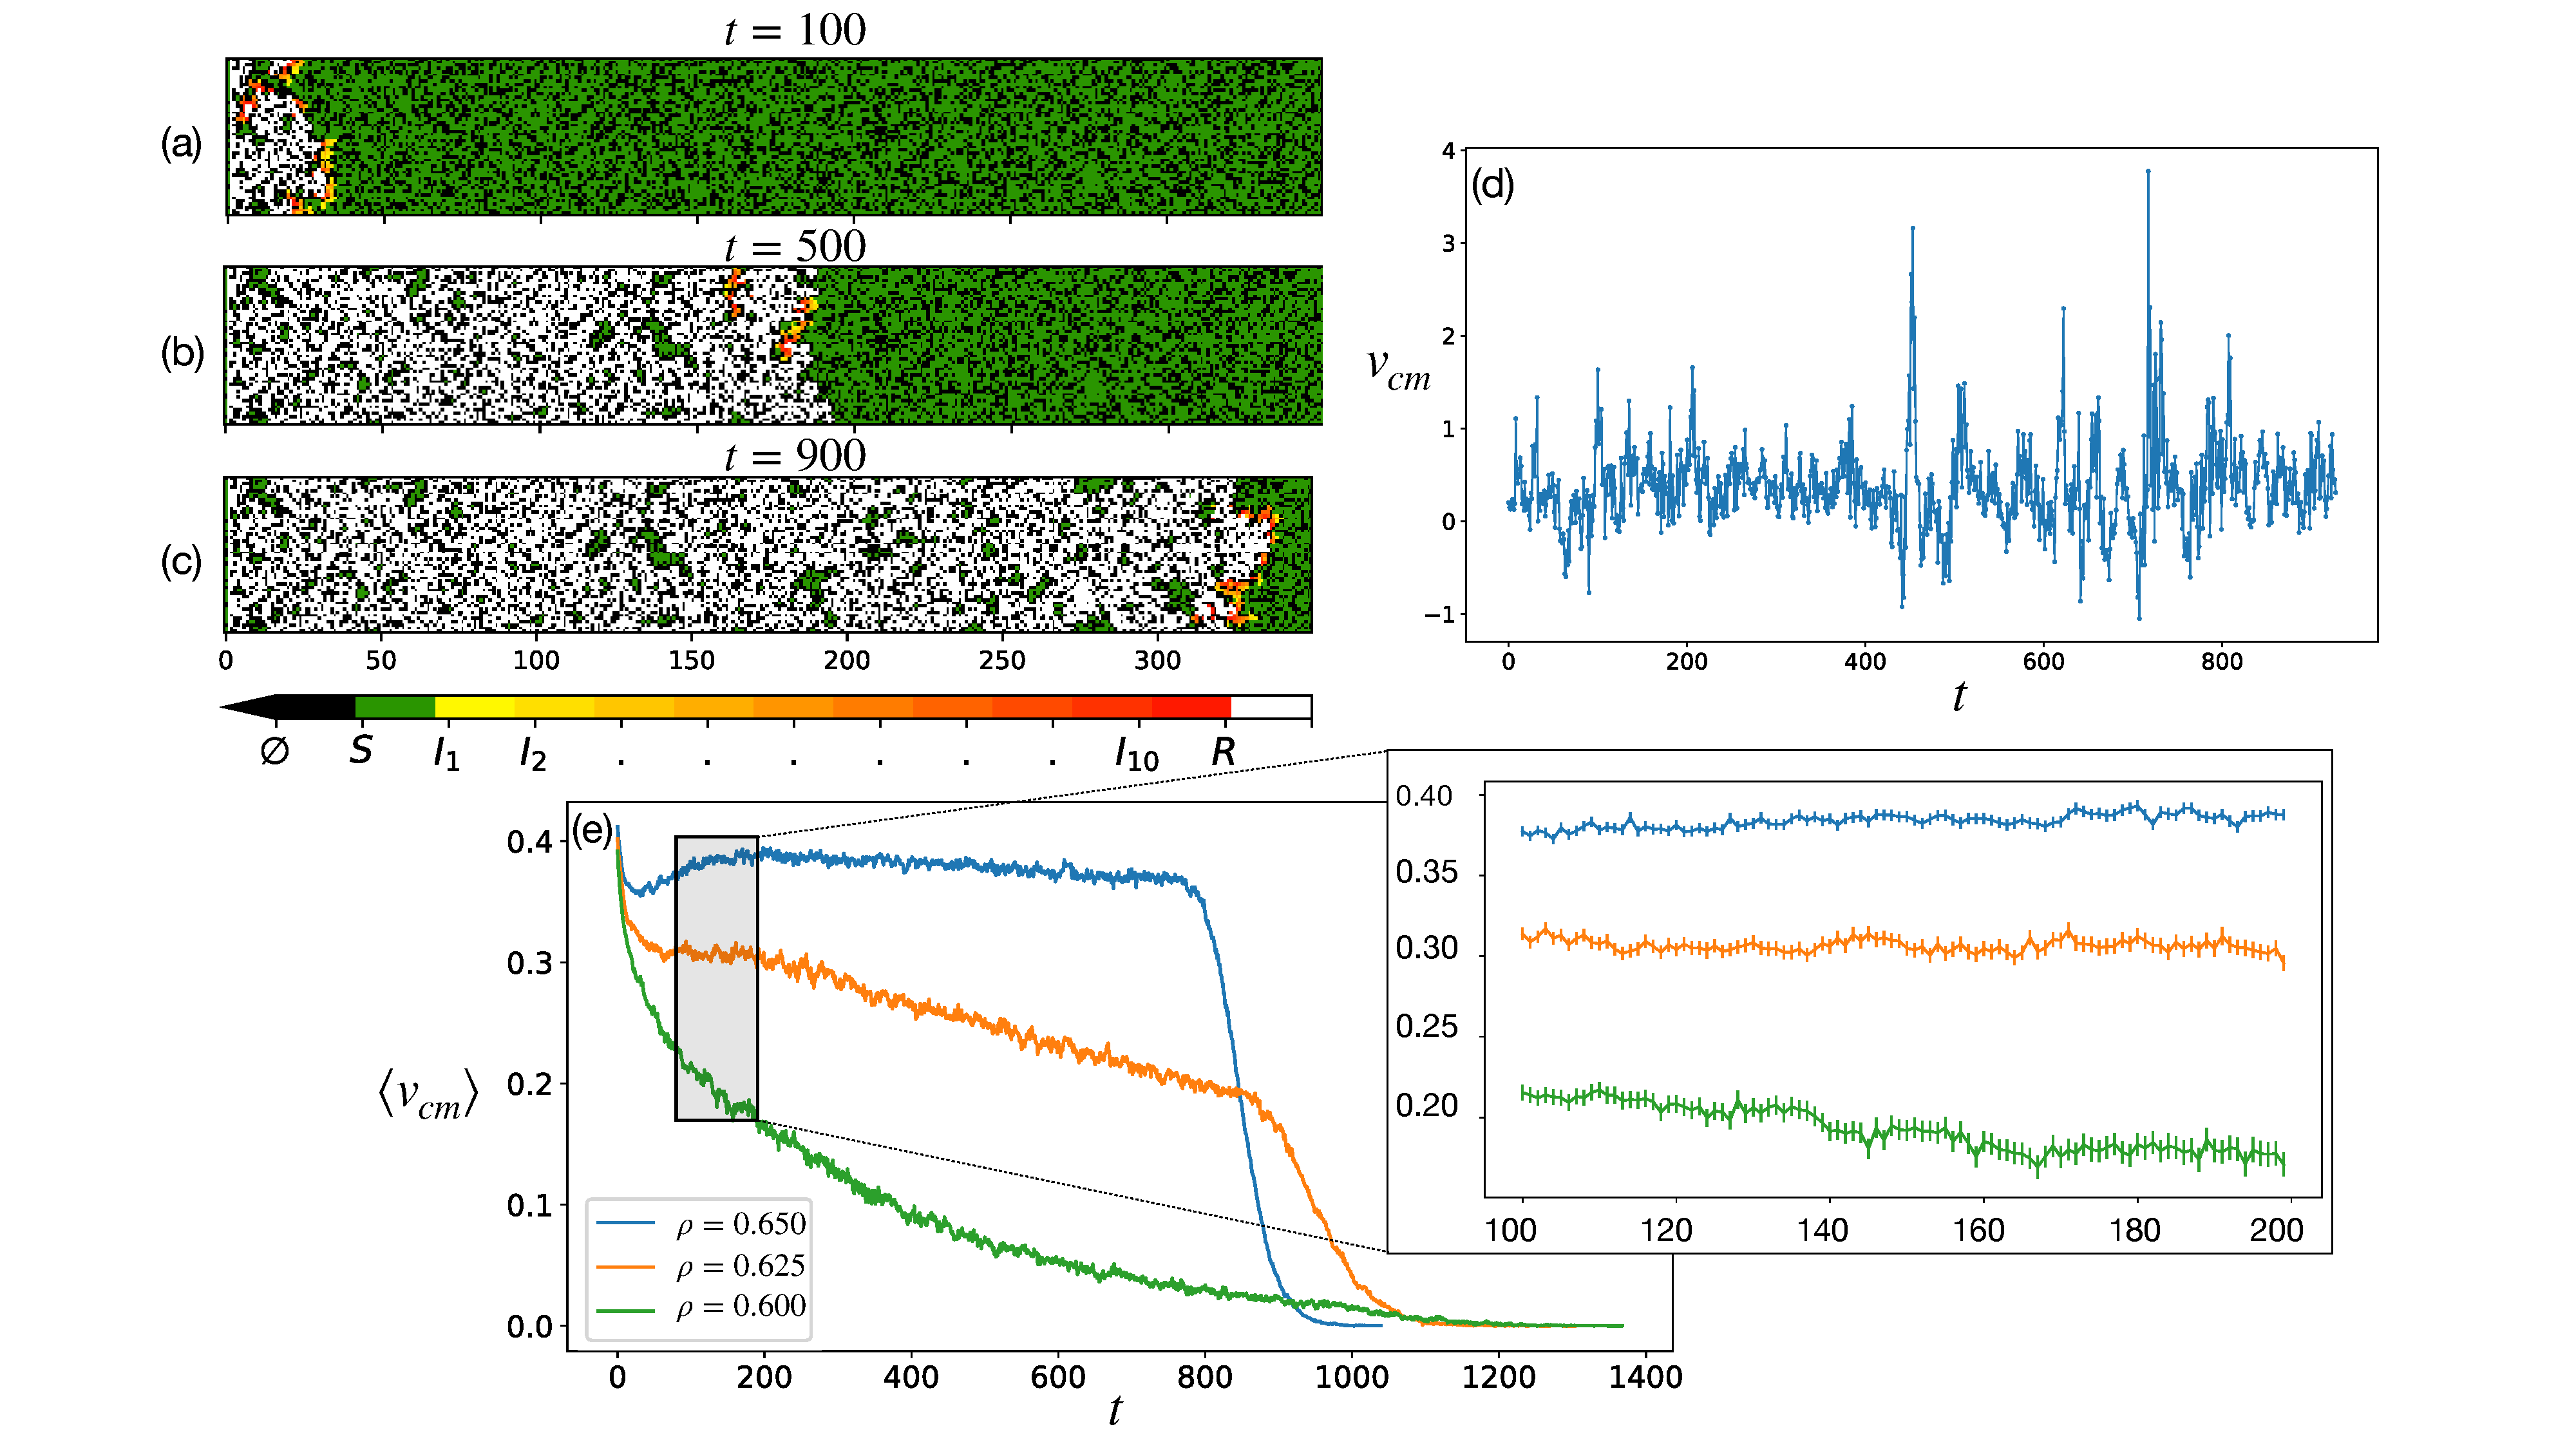
\includegraphics[scale=0.30]{chapter4/figures/figure1-channel-domain.pdf}
    \caption{
    (a-c) A channel domain of size $50\times350$ is shown over three time-steps for model parameters $\rho=0.65$ and $\beta=0.50$. 
    The centre of infectious mass is recorded for each time-step. 
    (d) Plots of the centre of mass time-series for the simulation illustrated in panels (a-c). 
    (e) The mean centre of mass time-series (of $10^4$ repeats) for three variations in density and $\beta=0.50$. 
    Time-series begins to decay around the mean simulation run-time.  
    The zoomed inset shows the ensemble averaged time-series for $t\in[100, 200]$ and reveals increases in error bars lower density parameters.
    }
    \label{fig:ews-primer}
\end{figure}

Consider a rectangular domain of size $[L_x, L_y]$ where $L_x>L_y$ and $(x, y)$ represent dimensions of width and height respectively.
Figures \ref{fig:ews-primer}(a-c) shows spatio-temporal spread in the domain, henceforth referred to as the `channel' domain, over three time-steps.
Epidemic parameters in the channel were arbitrarily chosen, yet lie above the threshold ($\rho=0.65$ and $\beta=0.50$).
The initial conditions required an adjustment from the square domain in Chapter \ref{chapter:SLM}, namely, the first column is infected and taken as the origin (denoted by $x_0$).
Additionally, the boundary conditions permit the disease to propagate freely in the $+x$ and $\pm y$ directions, thus realising a cylindrical geometry with periodic boundary conditions in $y$ direction and fixed boundary conditions in $x$.

We register a percolation event in the channel domain if an infected tree reaches the last column, denoted by $x_m$.
The percolation threshold shifts toward higher densities if the domain is sufficiently narrow (having a high aspect ratio), as the dimensionality of the travelling wave to somewhere between one and two dimensions\footnote{Additionally less space in computer memory is occupied and simulation time is lowered}. 
The higher percolation threshold can be understood by considering gradual increases in the domain aspect ratio, 
where, in the limit $L_y = 1$ and $L_x \gg 1$, a one-dimensional domain is realised and the critical host density increases to $\rho_c=1$.
In other words, increasing the aspect ratio eventually leads to the (higher-valued) one-dimensional percolation threshold.

Unsurprisingly, studies have confirmed that site and bond percolation (in $\mathbb{R}^2$ and  $\mathbb{R}^3$) depend non-trivially on a cylinders aspect ratio \cite{sangare2009continuum}.
Therefore, we choose an aspect ratio that approaches the percolation threshold for a two-dimensional square to keep consistent with the numerical results of Chapter \ref{chapter:SLM}. 
In practice, a channel of size $(L_x, L_y) = (350, 50)$, was sufficient, as shown through Figures \ref{fig:ews-primer}(a-c). 


\subsection{Centre of infectious mass}

The channel domain provides an advantageous setting to capture EWS by avoiding two-dimensional geometrical effects.
Moreover, the channel permits an improved (more intuitive) metric, based on the mean infective displacement from the origin:
\begin{equation}
   v_{cm}(t) = \frac{\sum^i x_i(t)}{N_I(t)} - \frac{\sum^i x_i(t-1)}{N_I(t-1)}
   \label{eq:COM}
\end{equation}
where $x_i(t)$ is the spatial location of the $i^{th}$ infected tree along the $x$ axis at time $t$ and $N_I(t)$ is the total number of infected trees. 
The form of Equation \ref{eq:COM} displays intrinsic similarities to the Newtonian center of mass:
 \[x_{cm} = \frac{\sum^i x_i\times m_i}{\sum_i m_i}\]
(where the analogous quantities in Equation \ref{eq:COM} are $m_i=1$ and $\sum^im_i= N_I$).
As such, the metric outlined in Equation \ref{eq:COM} will constitute a `centre of infective mass' (\acrshort{com}) velocity.
The COM time-series of Figure \ref{fig:ews-primer}(a) is shown in Figure \ref{fig:ews-primer}(b).
As opposed to the time series shown previously in Figure \ref{fig:vel_eff_rad_metric}(a), the COM metric looks different and allows for negative values.

Ensemble-averaged COM time-series $\langle v_{cm}\rangle$ are shown in Figure \ref{fig:ews-primer}(c) for the three values of tree density.
The blue time-series has epidemic parameters well beyond the threshold and begins to decrease around $t \in [800, 900]$, coinciding with percolation to the domain edge.
Contrarily, the green time series lies slightly above the percolation threshold and decays more gradually from $t=0$, due to a higher extinction probability. 
A small number of long-lasting simulations (exceeding $t>1000$ steps) occurred in the green time-series, indicating criticality in the system\textemdash 
previously likened to a regime of persistence in section \ref{sec:SLM-epidemic-threshold}.
The inset of Figure \ref{fig:ews-primer}(c) shows the ensemble-averages between $t\in [100, 200]$, including the standard error for each time-step.
Notably, error bars are most significant for the lowest-valued density shown in green, reflecting a more chaotic spread.

\subsection{Ensemble averaging method}

The findings of \cite{OROZCOFUENTES201912} were gathered by first producing a distribution of mean time-series velocities $\overline{v}_t$.
In this scheme, an EWS were detected from statistical moment-generation functions over the mean velocity, e.g. $\big\langle var(\overline{v_t}) \big\rangle $.
However, altering EWS detection by computing the mean simulation variance $ \big\langle \overline{var}({v}_t) \big\rangle $ was found to reveal a clearer signal.
Consequently, we proceed by detailing an ensemble method that permits the capture of `within-simulation' variance. 

Before the ensemble averaging method is elaborated, it makes sense to first define the relevant mathematical notation.
Suppose a simulation with parameters $\rho, \beta$ propagates for $f$ time-steps, Equation \ref{eq:COM} describes the time series as: $v_{cm}^{t=1}, v_{cm}^{t=2},..., v_{cm}^{t=f} \in V^{\rho\beta}$. 
Then, a set of $N$ independent time series are generated by repeating $N$ ensemble realisations. 
For an arbitrary point in the parameter-space ($\rho, \beta$),
the set of $N$ replicate simulations can be described by the set: \{$V_1^{\rho\beta}, V_2^{\rho \beta},..., V_N^{\rho\beta}\} \in \mathcal{V}_{\rho\beta}$, 
where each $V_i^{\rho\beta}$ describes an individual simulation time series and $\mathcal{V}_{\rho\beta}$ describes the entire ensemble for parameters $(\rho, \beta)$. 
Thus, an EWS is detected by calculating the mean time-series variance,
defined by:
\begin{equation}
\label{eq:ews_eq}
    \big\langle \overline{var}(v^{\rho\beta}_{cm}) \big\rangle = \frac{1}{N}\sum\limits_{i=1}^{N} var(V_i^{\rho\beta})
\end{equation}
A proper time-series analysis requires the same number of observations within each ensemble.
If not, we risk mistaking statistical fluctuations/errors for an EWS.
There are two observations to consider: 
(A) the number of time steps within simulations 
(B) the number of repeated simulations, $N$.

In general, stochasticity will prevent two simulations from having the same number of time steps, 
$|V_i^{\rho\beta}| \neq |V_j^{\rho\beta}|$.
Thus, calculating time-series variance for simulations with a small number of time steps might be more error-prone than long-lived simulations.
As such, we introduce a fixed window of time-steps ($t_O\leq t \leq t_F$) in a bid to fix the number of observations.
Provided the window length $t_F-t_O$ captures a sufficient number of time-steps, we avoid significant fluctuations in $V_i^{\rho\beta}$. 
Variance inside this window is defined by:
\begin{equation}
\label{eq:ews_eq1}
    \big\langle \overline{var}(v^{\rho\beta}_{cm}) \big\rangle = \frac{1}{N}\sum\limits_{i=1}^{N} var(V_i^{\rho\beta}\Big|^{t_F}_{t_O})
\end{equation}
Initial transience constrains the particular choice of $t_O$ in the channel, 
which distort calculations of the time-series variance. 
The lower bound was set to $t_0=100$ because initial instability occurred most over the first $100$ time-steps, and the window upper-bound to $t_F = 200$ (a two-fold increase of $t_O$) so that simulation variance is measured over a sufficient number of steps.
Lastly, the simulation boundary conditions required a slight alteration to fix the number of variance measures to $N$.
Previously, one of three events terminated a simulation, either: percolation, pathogen extinction, or when the number of time-steps exceeds the time horizon.
Here, we relax the condition that terminates simulations when the pathogen dies off;
otherwise, short-lived simulations ($t<t_O$) would be omitted from the ensemble and reduce the number of variance measures below $N$. 
Additionally, the time horizon is fixed to $t_F$, thereby mitigating the cost of simulating unnecessary steps.

\subsection{EWS parameter-sweeps}
\label{section:ews_slm}

Figure \ref{fig:ews-results} displays the mean time-series variance, as per Equation \ref{eq:ews_eq1}.
The colour bar shows variance over the entire parameter space of density and infectivity from white to back.
In Figure \ref{fig:ews-results}, the lower and upper red lines indicate a percolation probability of $Pr(\rho, \beta)=0.05$ and $Pr(\rho, \beta)=0.95$, respectively.
Inside these regions, the system transitions into an epidemic and we witness a considerable rise in the variance.

The observations of Figure \ref{fig:ews-results} agree with the results of \cite{OROZCOFUENTES201912}. 
Although measuring EWS over a two-dimensional parameter space reveals some additional information not captured in the original analysis, i.e. when infectivity is low ($\beta<0.40$), EWS preempt the epidemic by a more significant margin\textemdash indicated by the red arrows.
In addition, variance over the epidemic transition appears sharper when $\beta$ is high, as indicated by the darker shade in the upper right quadrant of Figure \ref{fig:ews-results}.

 \begin{figure}
    \centering
    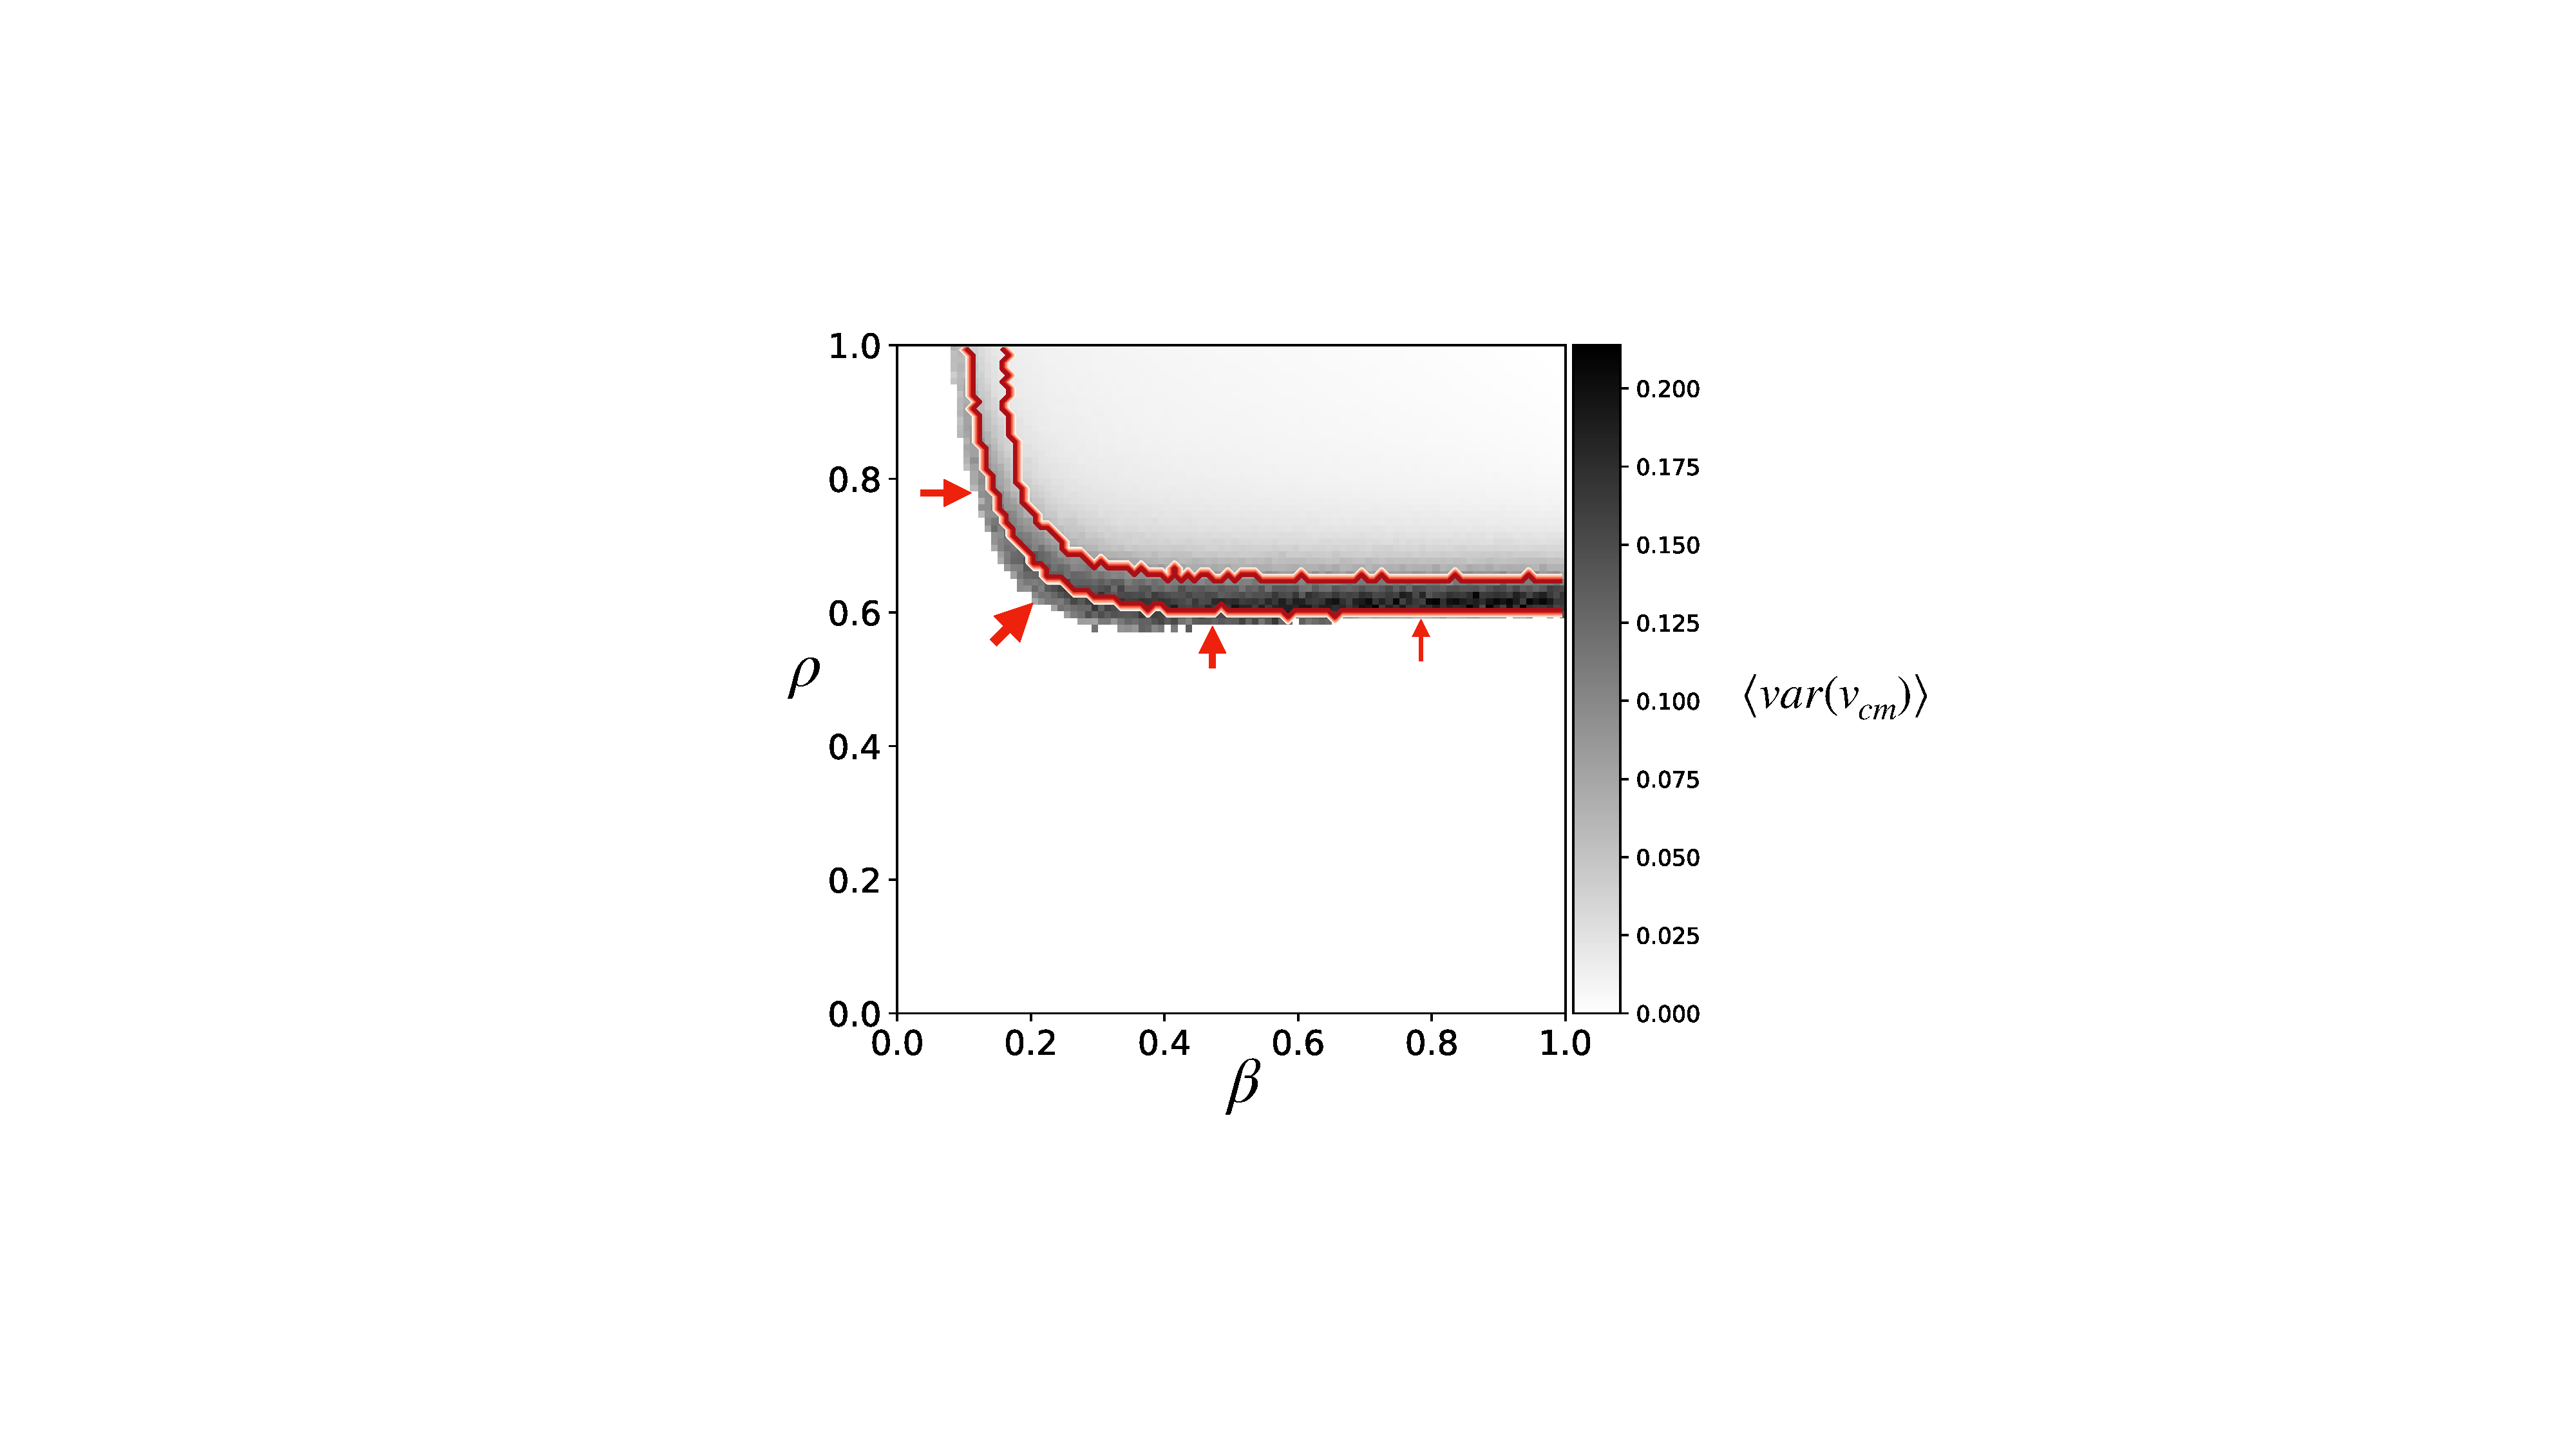
\includegraphics[scale=0.45]{chapter3/figures/figure11.pdf}
    \caption{The ensemble-averaged variance of $v_{cm}(t)$ over a two dimensional parameter sweep of $\rho$ and $\beta$. Red contours show the lower and upper bound of percolation (i.e. between $5\%$ and $95\%$ probability). 
     The epidemic regime is pre-empted by increases in variance more clearly for certain parameter values, %
     indicated by the arrows.}
    \label{fig:ews-results} 
\end{figure}

The following thought experiment can explain the EWS asymmetries in Figure \ref{fig:ews-results}: %
suppose infectivity is high, and density lies just below criticality ($\rho\lesssim\rho_c$), 
so susceptible clusters do not percolate. 
In this case, disease transmission is high on account of $\beta$, 
and all susceptible hosts become quickly infected, 
although an outbreak will come to a halt due to insufficient hosts. Therefore, in this model, 
an aggressive pathogen spreading through low tree densities may propagate rapidly but have a short, 
chaotic signature. Hence the transition is steep,
and the simulation variance is significant, as indicated by the smallest arrow in Figure \ref{fig:ews-results}. 
In this region, detecting an EWS is hard because transitions occur most rapidly.

Now we consider the converse, a less infectious pathogen with an abundance of susceptible hosts, 
located in the top-left region of Figure \ref{fig:ews-results}.
Here, transitions into the $I$ compartment are slower because the pathogen is less infectious, 
although this time, hosts are abundant.
Thus, a pathogen is likely to spread predictably for longer times, 
giving rise to a slightly less abrupt variance signature, 
as indicated by a lighter colour before the transition in the top left quadrant of Figure \ref{fig:ews-primer}.
Although the variance spike is not as significant, 
it preempts the epidemic transition by a more considerable degree\textemdash
indicated by the larger arrows in Figure \ref{fig:ews-results}.
Altogether, Figure \ref{fig:ews-results} indicates that the strength of an EWS depends on the particular combination of epidemic parameters, 
though fundamentally, an EWS is detectable for all parameter combinations.

\newpage

\section{Tree distribution datasets in Great Britain}
\label{ch2:hostdata}

Large-scale epidemic models of tree disease rest on robust, high-quality host data.
Data-driven approaches are crucial for predicting disease spread over country-wide scales, 
though collecting high-quality host data involves myriad challenges. 
Most notably, large-scale species distributions require vast datasets that demand significant economic resources
and person-hours to assemble and maintain over time. 
However, satellite-based remote sensing technologies pose an attractive solution\textemdash see \cite{camarretta2020monitoring} for a recent review of remote sensing technologies.
Despite the significant advances of remote sensing technologies, most freely available data sets still rely on traditional surveying methods to collect data throughout Great Britain (GB).
Consequently, the most widely known and widely used datasets are reviewed below.
Following this, statistically-generated species distribution models, typically based on surveyed data, are reviewed.

\subsection{National Surveys}
\label{sec:nationa-surveyes}

Surveyed data predominantly describes either: abundance, presence-only, presence-absence data. 
Generally, abundance data describes percentage canopy cover per $\mathrm{km^2}$.
In contrast, binary-valued presence-only and presence-absence data simply record if a species is present or present and absent, respectively.
Abundance captures significantly more information than presence-only data, yet unfortunately, they are in short supply.

\subsubsection{Countryside Survey}

The countryside survey (\acrshort{cs}) is a long-running, national survey of diversity and species abundance in GB \cite{wood2017long}.
The UK Centre of Ecology and Hydrology (UKCEH) undertakes the surveys, primarily funded by the Natural Environmental Research Council alongside other government agencies.
Individual surveys have been undertaken in: $1978$, $1990$, $1998$, $2007$, and $2019$. 
Random stratified sampling captures a representative species abundance\footnote{
A useful (unpublished) project merged abundance data from CS with myForest. The abundance data can be found at the Oxford University research archive: \nolinkurl{https://ora.ox.ac.uk}.} 
over of all land cover compositions, e.g. lowland acid grassland, freshwater, and broad-leaf forest.

Abundance data is collected for numerous dominant species, including trees, shrubs, ground flora and soil type, 
making the scope of CS data vast. Moreover, long-running records spanning decades reveal ecosystem trends imperative for ecological monitoring.
More recently, $100$ $1\mathrm{km^2}$ plots of vegetation and soil data were collected\footnote{
The data is free to download on the UKCEH website: \nolinkurl{https://catalogue.ceh.ac.uk}} \cite{10.5285/fd6ae272-aeb5-4573-8e8a-7ccfae64f506}.
The dataset constitutes the first of five planned surveys, part of a rolling monitoring strategy collected every five years.

\subsubsection{National Forest Inventory}

The National Forest Inventory (\acrshort{nfi}) collects and maintains forest and woodlands data in GB.
Originally, the NFI was established to help restore and expand Britain's woodlands following the First World War \cite{james1990history}.
Regular programs ($10$-$15$ year intervals) implement surveys of woodland and forest size, distribution, composition and condition across GB.
Records cover areas over $0.5\ \mathrm{ha}$ and $20\%$ coverage.
As of $2019$, $622,381$ individual records exist, spanning $2.9 \times 10^6\ \mathrm{ha}$ over $13\%$ of the total land cover within GB.
NFI data comprise ESRI shape files\footnote{
Free to download at: \nolinkurl{https://data-forestry.opendata.arcgis.com}},
that outline numerous forest types, e.g. broadleaved, conifer, mixed-predominantly broadleaved or mixed predominantly conifer.
Despite an extensive coverage, publicly available NFI surveys describes presence-only data\textemdash with no proportion or species coverage.
Although, additional datasets are available to purchase, including: 
(1) Tree species percentage per region by woodland type
(2) Tree species proportions within the upper canopy of each NFI sample plot, without supplying the exact location of the individual sample plot.

\begin{figure}
    \centering
    \includegraphics[scale=0.2]{chapter2/figures/NFI-figure.pdf}
    \caption{NFI data super imposed onto a Google earth image, taken from a report (unpublished) by S. Orozco-Fuentes et al.
             NFI data covering Thetford Forest Park ($16.684 \mathrm{km}^2$) is shown as a polygon in the NFI `woodland' category.
             Data is interpreted as the conifer forest type. Here, surveys comprises presence-only data, and no tree species percentage cover
             is reported. NFI data extends throughout $\sim 13\%$ of land coverage in GB and large non-woodland areas remain un-surveyed.}
    \label{fig:NFI-data}
\end{figure}

\begin{figure}
    \centering
    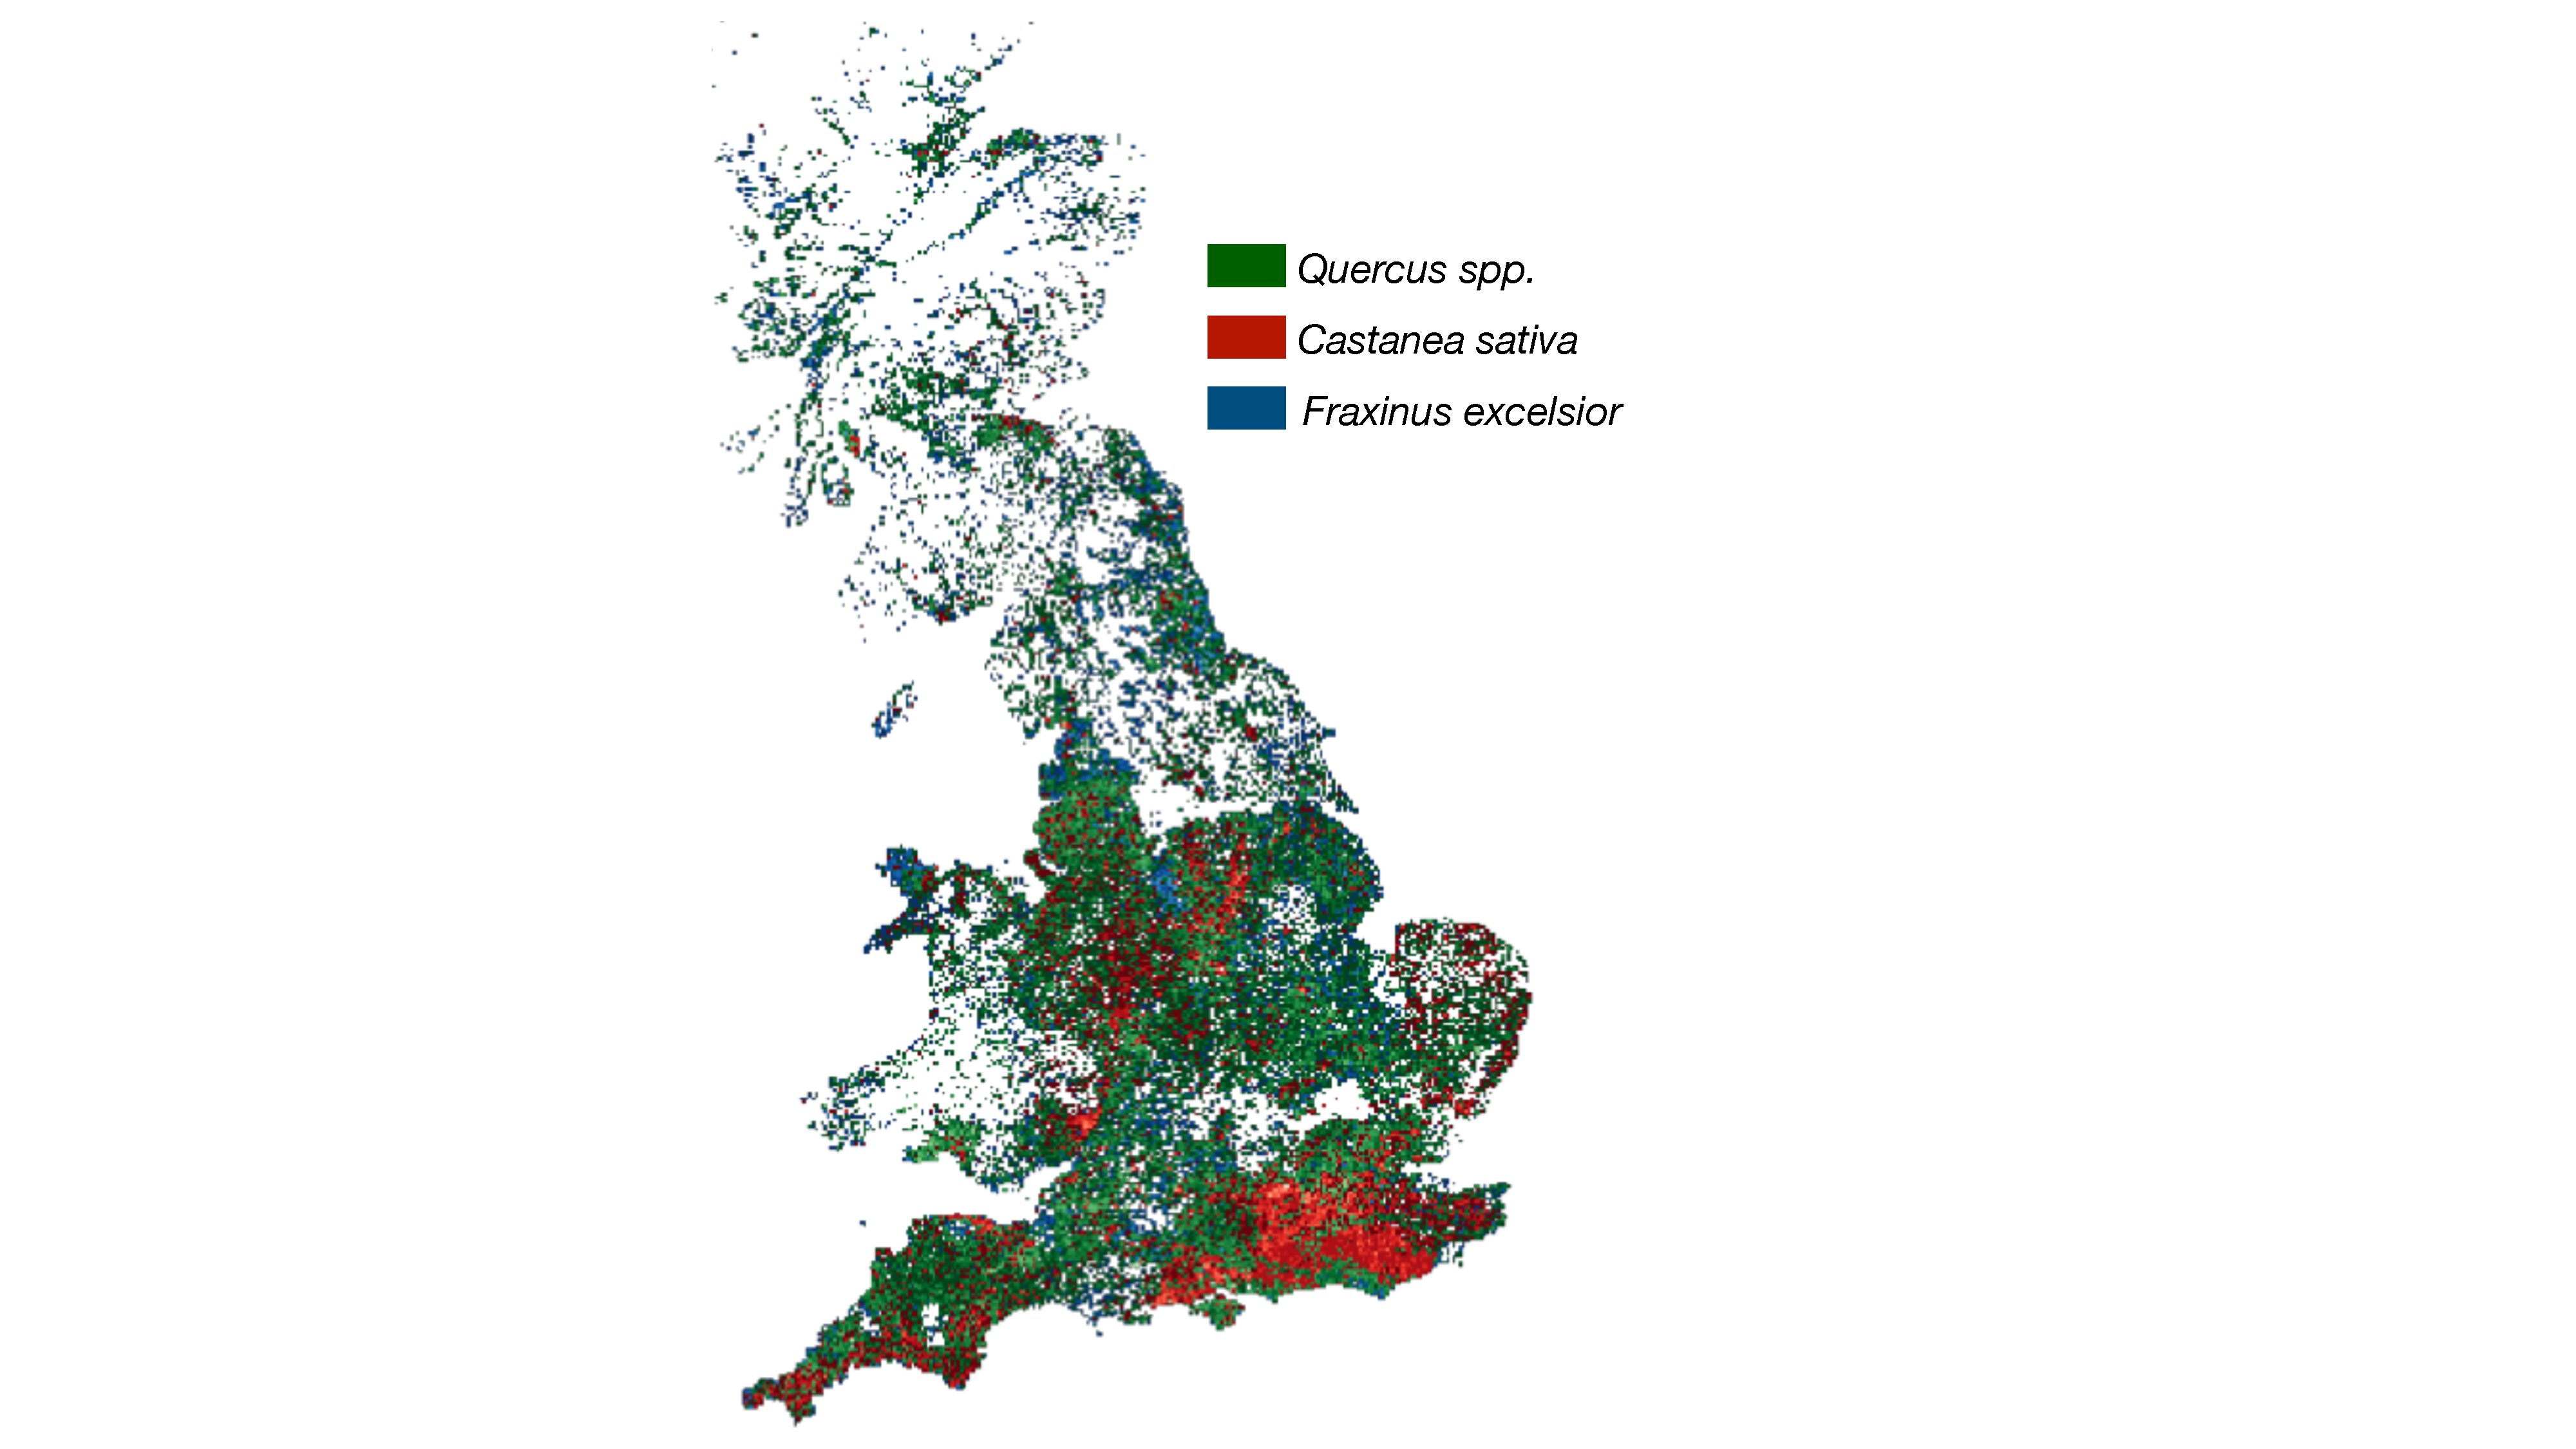
\includegraphics[scale=0.25]{chapter2/figures/bsbi-data.pdf}
    \caption{BSBI presence-only datasets\textemdash as reconstructed by S. Orozco-Fuentes et al. (unpublished).
    Three important large deciduous tree species, European ash (\textit{Fraxinus excelsior}), 
    Oak (\textit{Quercus spp.}), and sweet chestnut (Castanea sativa), are overlaid onto the same map at $\mathrm{2km \times 2km}$ resolution.
    The BSBI datasets are extensive and report presence-only data over a country-wide scale.
    }
    \label{fig:bsbi-data}
\end{figure}

\subsubsection{Botanical Society of Britain and Ireland}

The Botanical Society of Britain and Ireland (\acrshort{bsbi}) has recorded species presence-only data since $1950$.
BSBI datasets are publicly available\footnote{BSBI data can be downloaded from: \nolinkurl{https://database.bsbi.org}.} upto a
resolution of $\mathrm{2 km \times 2km}$, though records upto $\mathrm{100 m \times 100 m}$ are available to registered members.
As of $2020$, BSBI records are collected at $\mathrm{1 km \times 1km}$ square resolution or better\textemdash making the datasets among the 
highest-resolution surveys collected by traditional methods. The BSBI distribution database contains records of plants and charophytes
as reported by users and conservationists with MapMate\footnote{MapMate is software designed to aid users to share ecological data: \nolinkurl{https://www.mapmate.co.uk}}.
Despite the availability of high-resolution data, observations are collected ad hoc by users and not curated scientifically.
Moreover, the distributions contain both well-surveyed and poorly-surveyed plots of land likely to carry uncertainties.
As such, BSIBI data is helpful to reconstruct several baseline tree distributions across GB, as demonstrated by \cite{hill.data}.

\subsection{Species distribution models}

In the absence of extensive host data, species distribution models (\acrshort{sdm}s) aim to generate synthetic data, typically from less-extensive surveys.
SDMs were first developed in the $1990$s, and have subsequently become fundamental to ecological and biogeographical inference studies.
Synthetic distributions have been used to examine biodiversity, conservation, resource management, 
ecology and climate change \cite{franklin2013species, skov2016real, wittmann2016confronting, 10.3958/059.037.0110, zhang2019using}.
The vast majority of SDMs fall into two categories: correlative \cite{srivastava2019species}, and mechanistic \cite{shabani2016comparison}.

Correlative SDMs relate (widely available) presence-only, or presence-absence, data to several environmental predictor variable datasets.
For tree species, predictor variables include temperature, precipitation, altitude, and soil type \cite{ray2021multi, hill.data}.
Following this, a species distribution map can be predicted, albeit with  uncertainties and errors.
Commonly used statistical methods include Regression 
(i.e. General Linear Models, General Additive Models, Multivariate Adaptive Regression Splines) and Machine Learning
(i.e. Artificial Neural Networks, Classification And Regression Tree, Random Forest). 
The general correlative approach is reflected in Figure \ref{fig:sdm}; for a more in-depth review of correlative SDMs, see \cite{SDM_1}.

Correlative SDM approaches require little to no prior knowledge of the physiological processes that link organism and environment.
Hence, mechanistic methods aim to incorporate an organisms behavioural, physiological, and morphological constraints to the environment, 
as reviewed by \cite{kearney2009mechanistic}. However, linking a species physiological response to the environment comes with significant
computational challenges, as it typically relies on vast, multi-variable time-series datasets \cite{shabani2016comparison}.

\begin{figure}
    \centering
    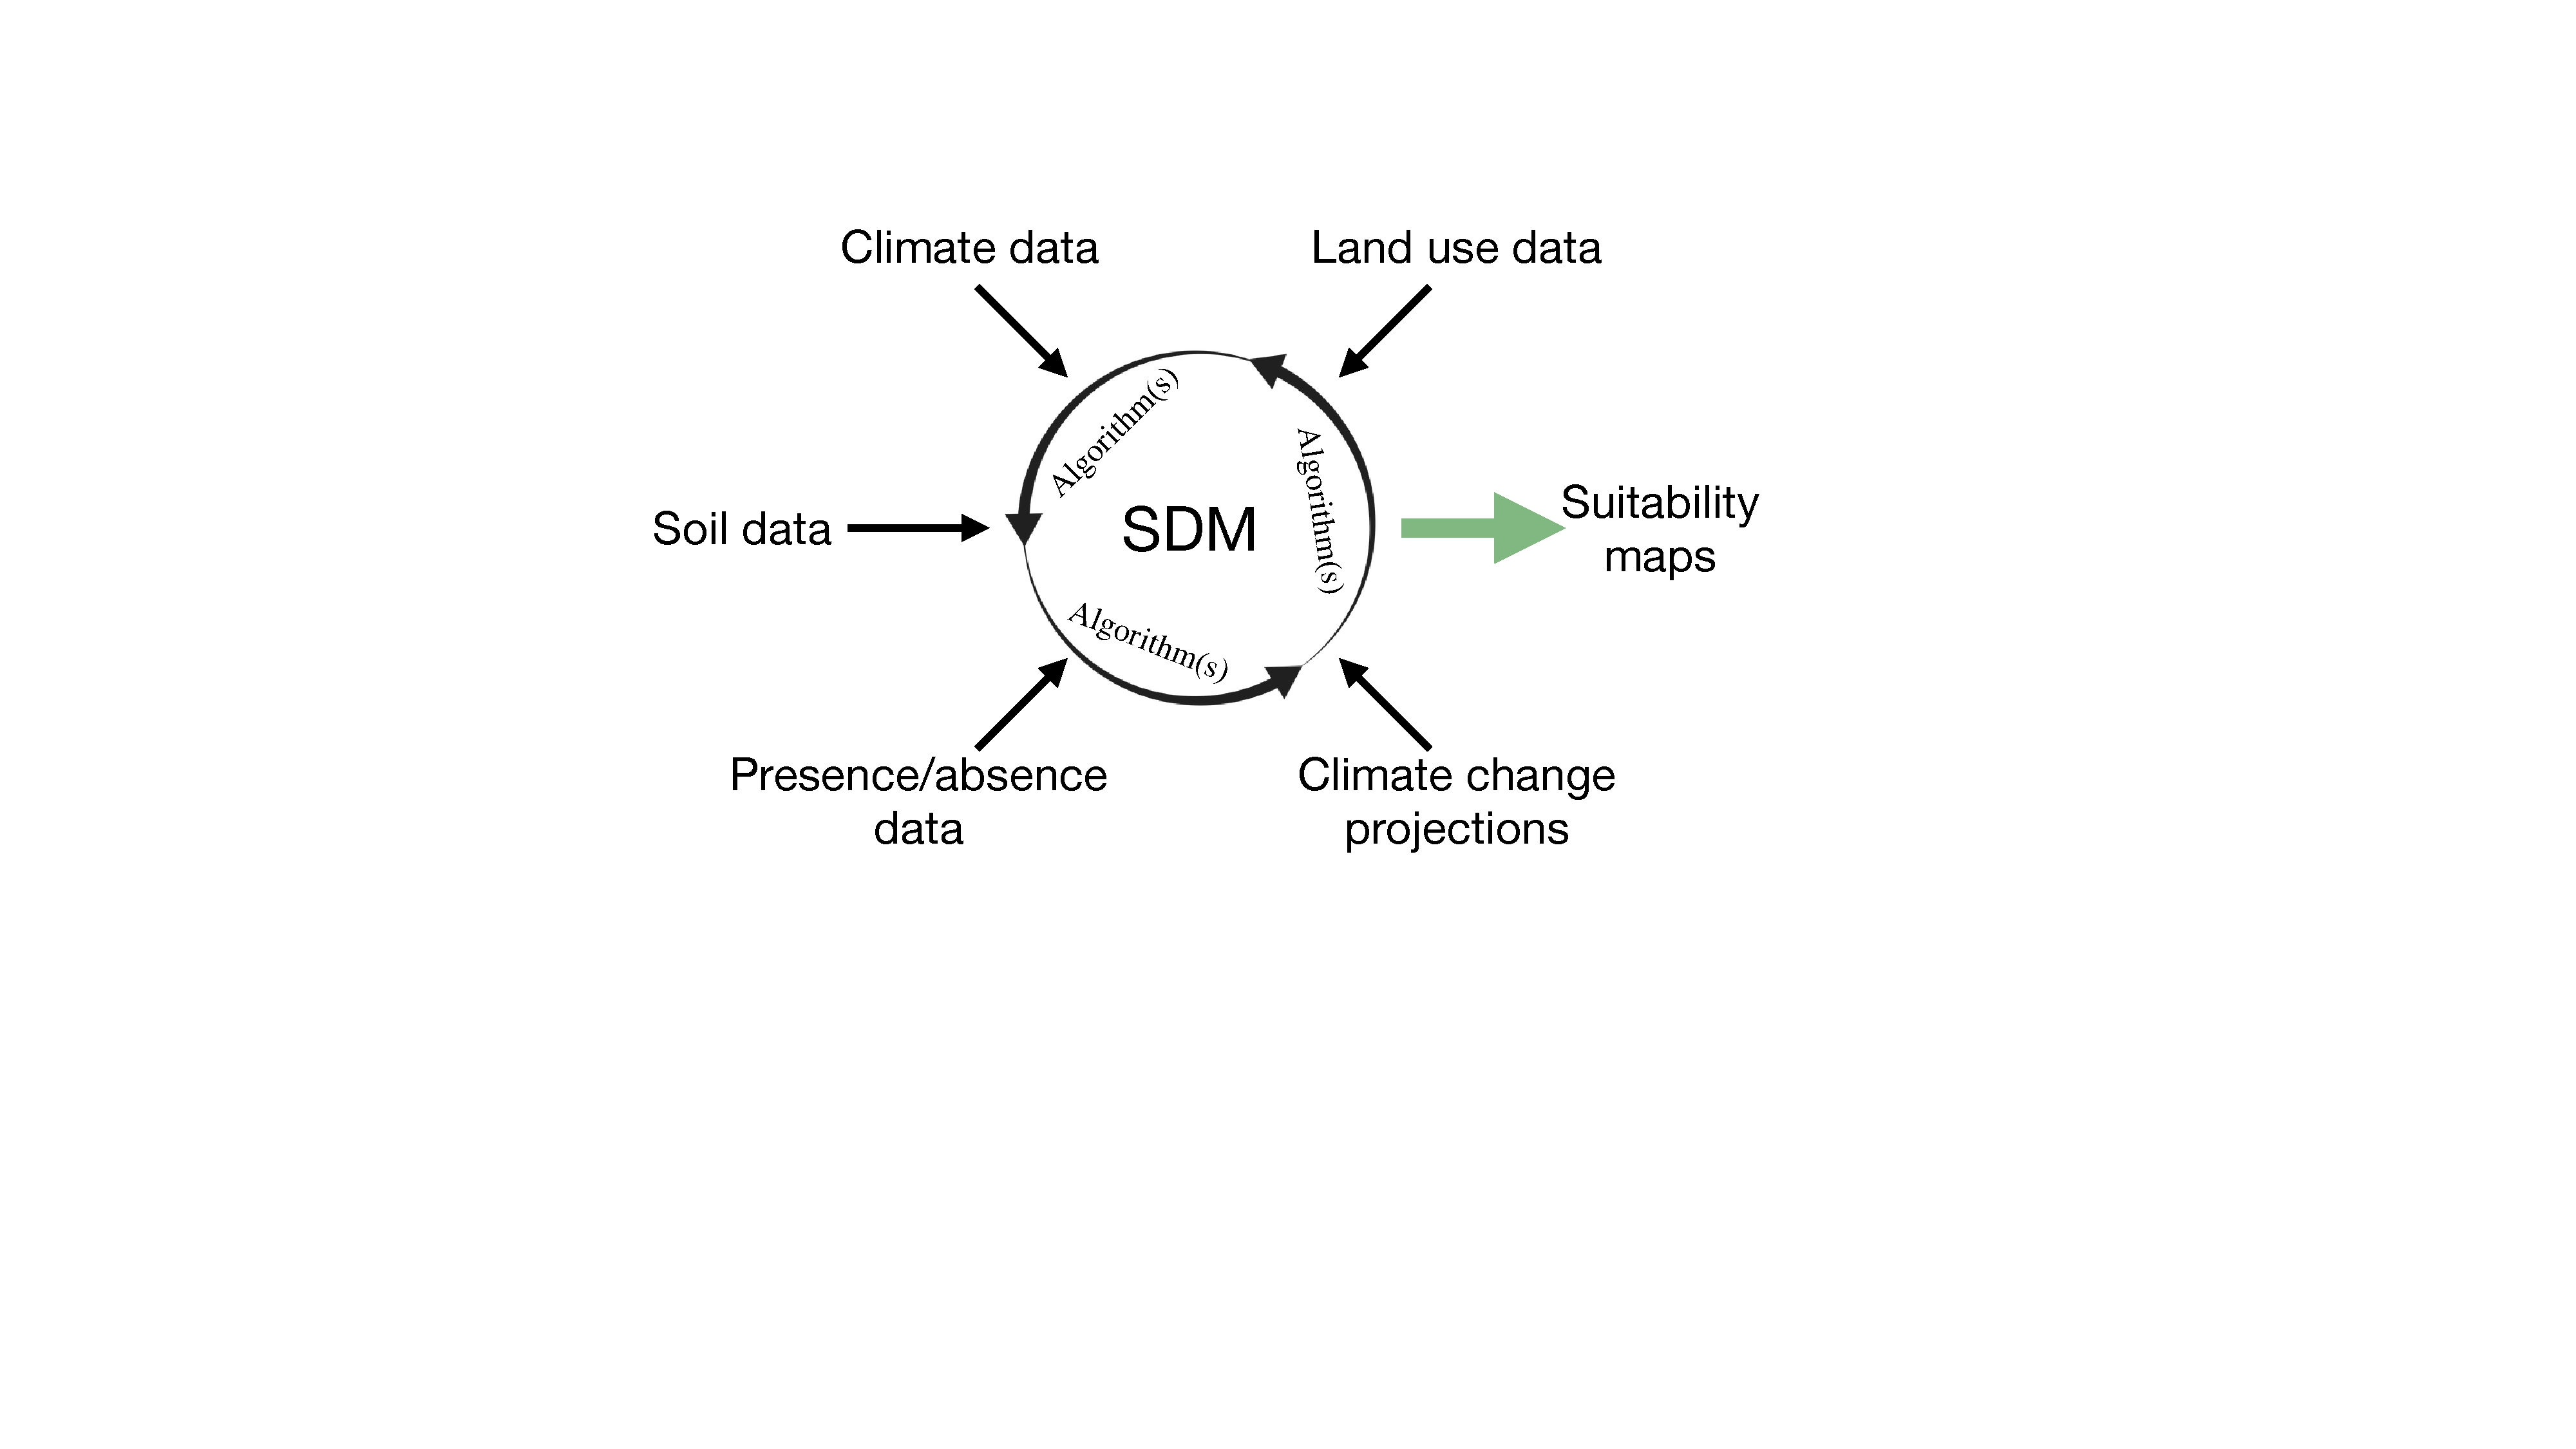
\includegraphics[scale=0.35]{chapter2/figures/SDM-fig.pdf}
    \caption{A graphical species distribution model (SDM) illustration, adapted from \cite{SDM_1}. 
             A variety of predictor variables and input data sources are used in conjugation with modelling algorithms to produce
             a habitat suitability map.}
    \label{fig:sdm}
\end{figure}

A review paper by \cite{guillera2015my}, revealed a diverse use of SDMs.
Out of $100$ publications reviewed by \cite{guillera2015my}, SDMs were applied to: 
(1) managing threatened species ($16\% $ of articles) 
(2) predicting climate change impacts ($13\%$) 
(3) understanding phylogeographic patterns ($9\%$) 
(4) controlling threatening processes ($8\%$) 
(5) landscape management ($8\%$) 
(6) biological invasions ($7\%$). However, no epidemic applications were reported.

Nevertheless, a thorough literature search revealed a variety of epidemiological SDM applications.
The crossover between ecological SDM methods and epidemiology has been referred to as `Infectious Disease Cartography' \cite{KRAEMER201619}.
With Infectious Disease Cartography, one seeks to map the likelihood, or risk, of infectious disease outbreaks and produce risk-maps.
A number of publications have applied SDMs livestock diseases \cite{hollings2017species}, and human-based diseases including the global 
distribution of Dengue Fervour \cite{bhatt2013global} and Zika virus \cite{messina2016mapping}, and Anthrax in Kenya \cite{otieno2021modeling}.
However, SDM applications for tree disease epidemics appear absent from the literature.

\subsubsection{Predicting species abundance}

SDM-generated tree occurrence data have limited applications to ecologists and forest managers.
This motivates statistically-generated abundance data that includes significantly 
more information about the population occupation/density and ecosystem.
Modellers have examined numerous approaches to predict tree species abundance;
including, linking the abundance-occupancy relationship \cite{gaston2000abundance} and
the scaling pattern of species occupancy over progressively smaller spatial scales \cite{hui2009extrapolating}.

An interesting, and highly relevant, approach to predict the abundance of common tree species in Great Britain was put forward by \cite{hill.data}.
At a high level, BSBI presence-only data were combined with a series of environmental covariates using a species distribution model to 
produce a map of predicted occurrence data. Then, random forest regression was employed with a training sample ($70\%$) of less extensive abundance 
data (consisting of CS, myForest and Bluesky's National Canopy Map). 
Results were then cross-validated with the remaining ($30\%$) abundance data; Figure \ref{fig:hill-method} displays a
flow-diagram of the method presented by \cite{hill.data}. 

A more detailed explanation of the treatment proposed by \cite{hill.data} follows:
\textbf{Stage (1)}
\textit{
\begin{itemize}
    \item Presence-only BSBI data was downloaded for $25$ common species of trees in GB, 
    and all records less than $\mathrm{2km \times 2km}$ resolution were discarded.
    Next, the presence-only data was converted into presence-absence data by considering
    `well-surveyed' records that Hill et.al defined as having a minimum of two survey
    between $1950$ and consisting of $50$ species. Species missing from these 
    well-surveyed areas were assumed truly absent. 
    \item Using biomod2 \cite{thuiller2016package}, a SDM was then fitted against a cohort of 15 environmental variables, e.g.
    soil type (European Soil Database), temperature (Worldclim), precipitation (Worldclim), altitude (Worldclim),
    type of land cover (Countryside Survey), among others. The net result was a map of predicted occupancy at $\mathrm{1 km \times 1 km}$ 
    resolution.
    \item For each species, predictions from a suit of models\textemdash GLM, GAM, CTA, GBM, RF\textemdash were
    repeated and combined into an ensemble distribution model. Each model was cross-validated against
    $30\%$ of the well-survyed BSBI presence-absence data using the receiver operator curve (ROC) \cite{jimenez2012insights} and the true skill statistic (TSS).
    \cite{hill.data} then selected the best performing predicted occurrence for each species.
\end{itemize}
}
\textbf{Stage (2)}
\textit{
\begin{itemize}
    \item Abundance data from CS and myForest were both expressed as hectares covered per kilometer 
    squared ($\mathrm{ha/km^2}$). This entailed using woodland cover from the NFI dataset to multiply
    the percentage cover of each species within a woodland patch, with a proportion of woodland cover per kilometer.
    \item Random forest (RF) regression then modelled the relationships between (CS and myForest) abundance data with
    the SDM-generated map of predicted occupancy. In addition, RF regression used four covariates, 
    three of which consisted of Bluesky's National Canopy data (i.e. total tree cover, woodland tree cover, non-woodland tree cover)
    and NFI edge broadleaved woodland (i.e. within $50\mathrm{m}$ of non woodland) data.
\end{itemize}
}

The abundance datasets produced by \cite{hill.data} combine several mainstream tree datasets in GB; moreover, 
constructing the ensemble model involved a variety of statistical models.
The predicted occurrence data was examined against the ROC.
Most species demonstrated functional ROC scores between $0.71$ and $0.96$ and performed exceptionally
well for ash ($0.96$) and oak ($0.90$).  

Although there were numerous assumptions that underpinned the methodology.
Primarily, the BSBI dataset used by \cite{hill.data} exists through ad-hoc user and volunteer self-reports.
Thus, some regions are more surveyed than others over time, which led Hill et al. to make the 
`well surveyed' recorded assumption (i.e. only considering records surveyed twice since $1950$ containing a minimum of $50$ species).
The assumption permitted the conversion of raw presence-only to presence-absence, 
at the cost of overestimated absence in these regions. That is, even supposing $50$ species
are reported within a subset of the ($\mathrm{2km \times 2km}$ tetrad) record, other large regions could remain unsampled\textemdash
the authors did not appear to scrutinise this assumption sufficiently.

\begin{figure}
    \centering
    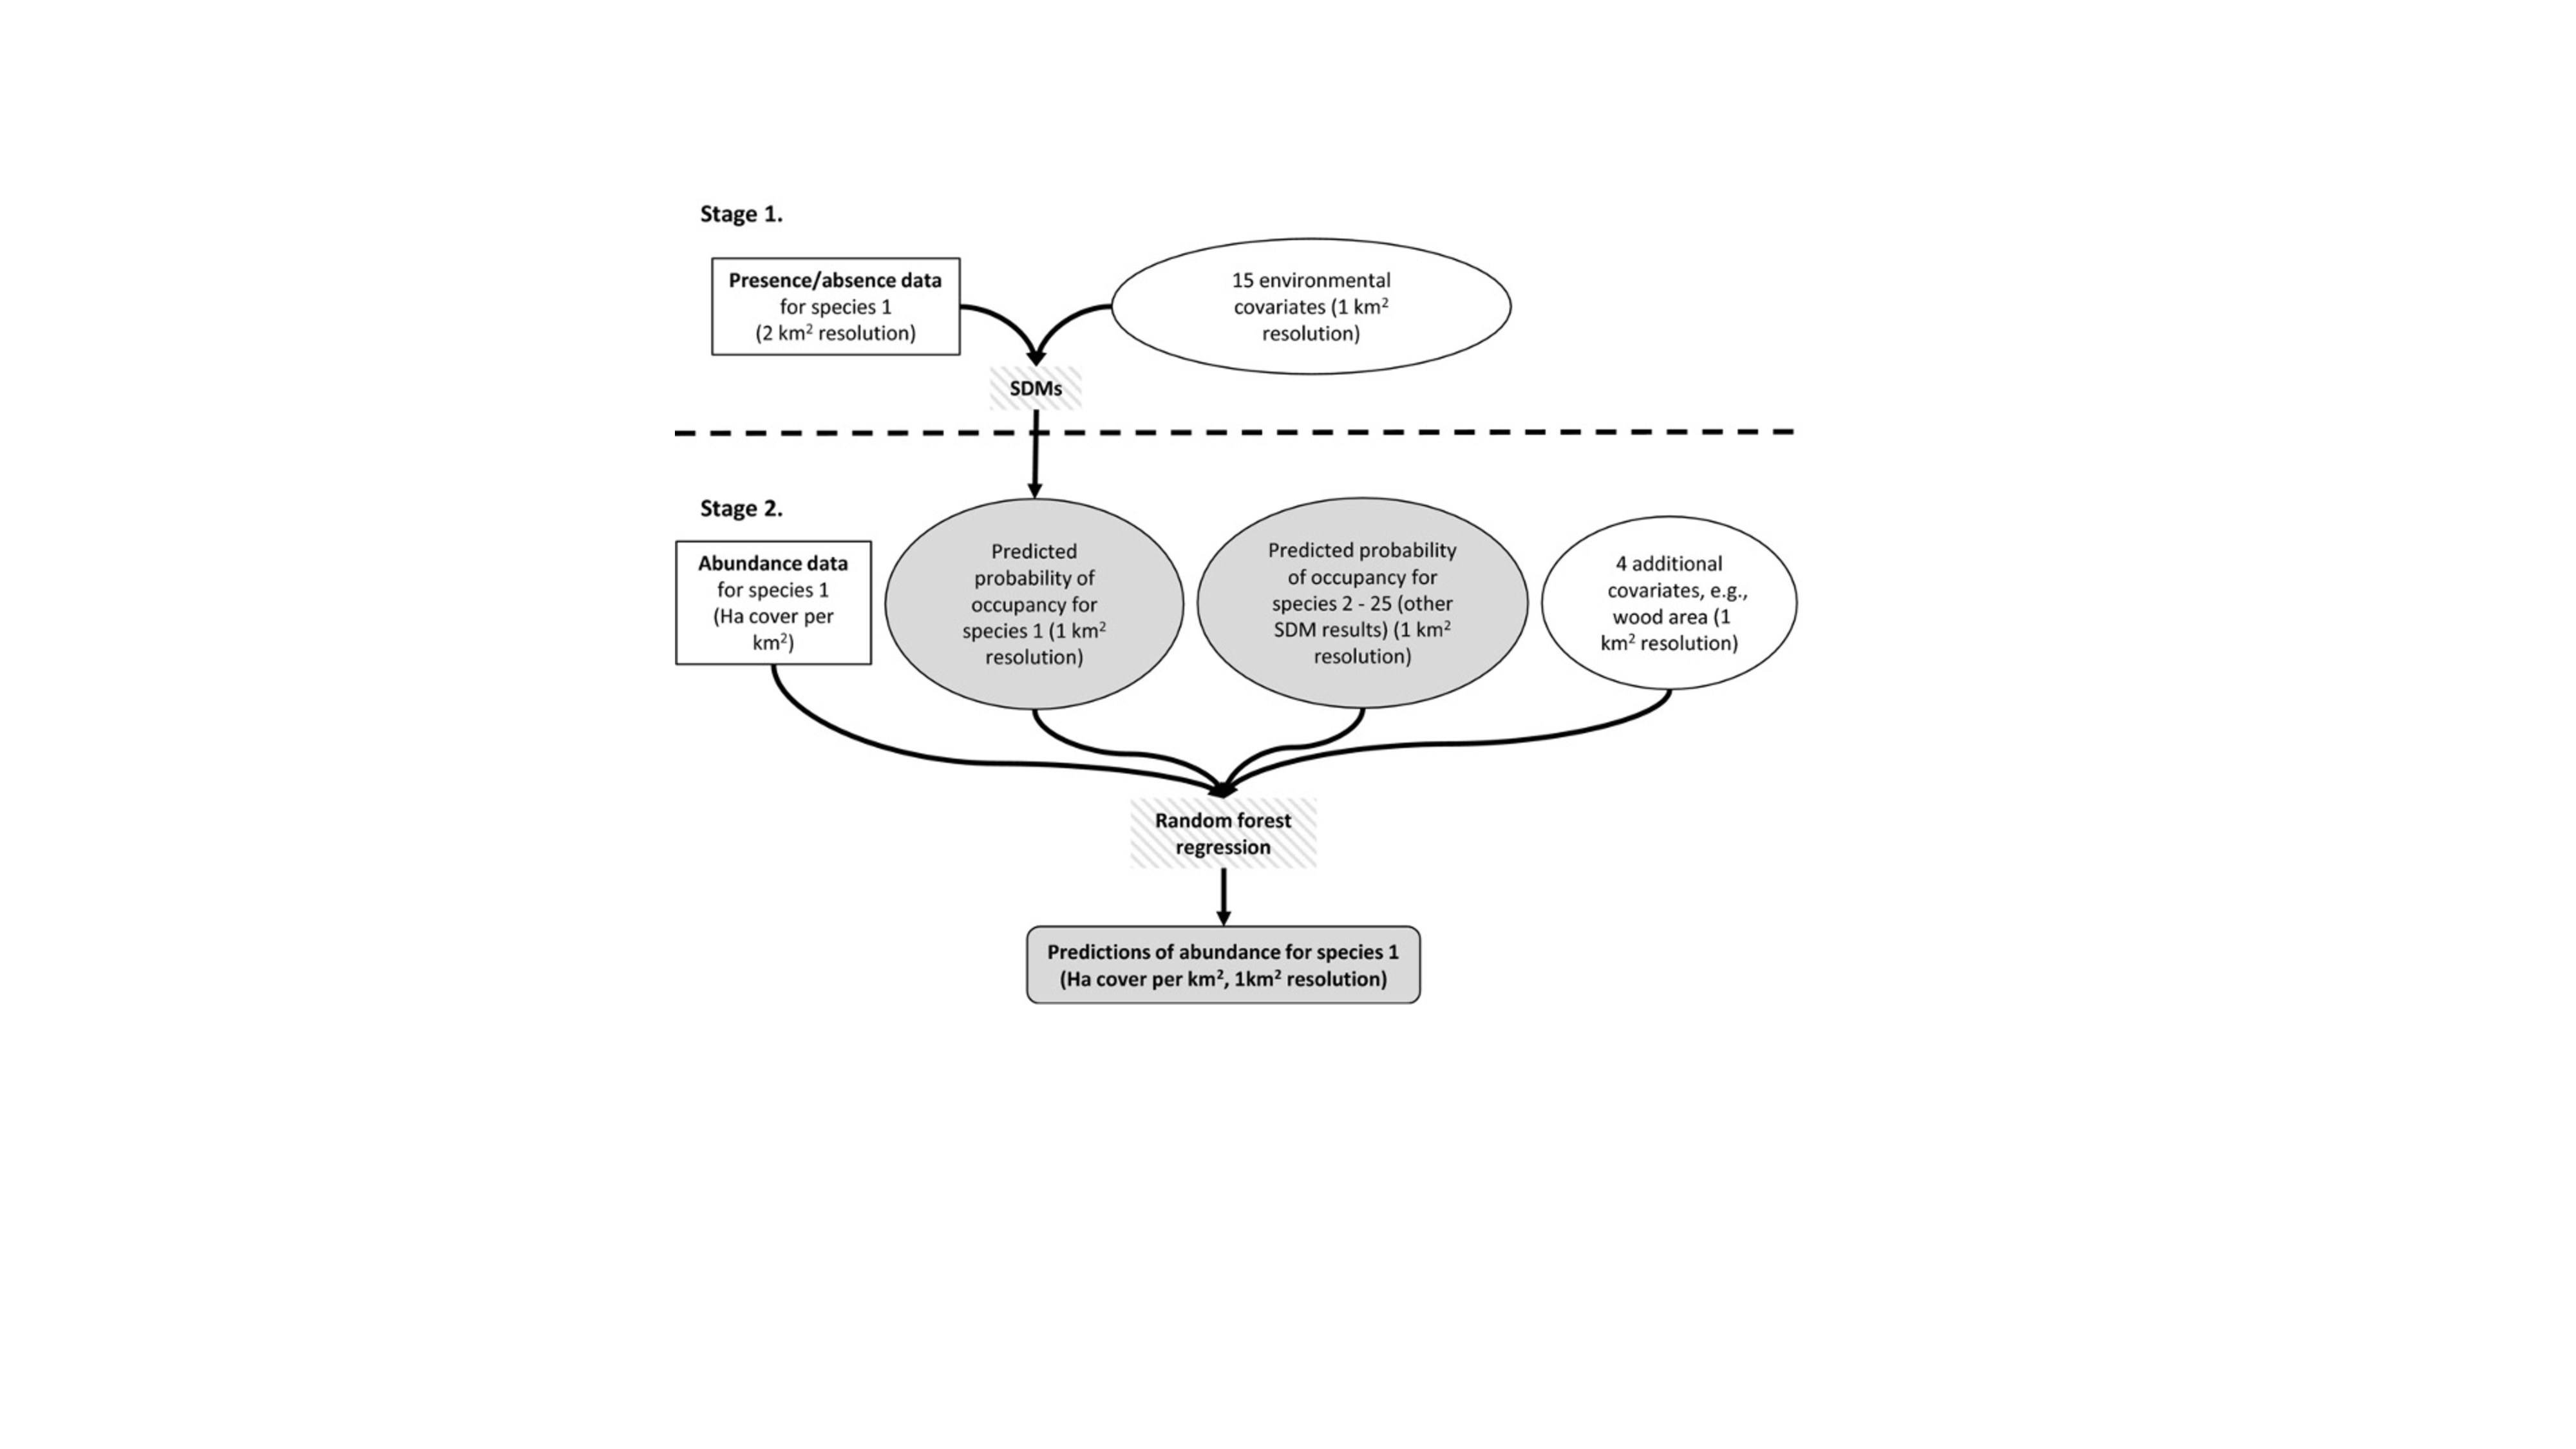
\includegraphics[scale=0.55]{chapter2/figures/hill-method-fig.pdf}
    \caption{A flow diagram of the two-stage abundance method put forward by \cite{hill.data} to model tree species abundance  
    (taken from the publications' materials and methods section).}
    \label{fig:hill-method}
\end{figure}

The RF regression used by \cite{hill.data} marked a novel approach to modelling species abundance.
The authors chose to argue in favour of RF regression because of its insensitivity toward the data distribution,
which worked well with the less comprehensive abundance data sources (as the map of abundance had a high percentage of zeros from missing records).
The abundance model quality was examined against $10$-fold validation (explained in \cite{refaeilzadeh2009cross}).
The root-mean-square error (\acrshort{rmse}), between predicted and observed abundance, generally ranged between $5$ and $10$,
where the RMSE scale reflects the response variable units ($\mathrm{ha/km^2}$), i.e. $5\%$ and $10\%$ respectively.
The result was country-wide predicted abundance, with noticeable, yet sufficiently low inaccuracies.

The low amount of available abundance data in GB significantly impoverished the abundance maps produced by \cite{hill.data}. 
Consequently, of the $25$ species datasets considered, all will contain numerous (small-scale) errors and uncertainties. 
Nonetheless, the modelled abundance maps captured more large-scale spatial structures than both the BSBI and CS distributions.

More recently, \cite{ray2021multi} produced a similar SDM as Hill et al. for oak in GB using biomod2 \cite{thuiller2016package}.
The authors focused on mapping high-density oak woodlands (with 60$\%$ canopy cover or above) 
to predict which NFI map polygons (by forest type) were most likely to contain oak stands. 
However, \cite{ray2021multi} did not make their oak maps publicly available, nor did they produce a general-purpose
abundance map relevant for epidemiological studies. 
To date, the data sets produced by \cite{hill.data} constitute the best publicly available
country-wide maps of abundance in GB, despite their limitations.

\newpage
%\item remote sensing tools were used \cite{kelly2002monitoring} to track the study of sudden oak death in California
%\item \cite{kelly2002landscape} demonstrated clustering at the landscape level, spatial structure is important

\section{A toy landscape-level SLM}

So far, this work has focused on a homogeneous distribution of hosts randomly populating an ideal domain. 
In this section, a toy landscape-level SLM is constructed and simulated on the map of Great Britain (GB).
Modelling the spread of disease over GB entails a large change of scale within the SLM. 
Specifically, host units now comprise $\mathrm{1km \times 1km}$ `\textit{patches}' of land. 
Collecting high-quality abundance data over large areas is challenging and expensive\textemdash reviewed in section \ref{ch2:hostdata}.
Therefore, the SLM is combined with a map of predicted oak abundance produced by \cite{hill.data}.

\subsection{Realistic boundaries}

Realistic host distributions describe complicated, irregular and heterogeneous domain boundaries
known to influence the spread of disease \cite{madden1995plant}.
In contrast, the SLM spreads through a square lattice with regular domain boundaries and homogeneously distributed hosts.
Moreover, the initial conditions (ICs) in the SLM have been limited to a small \textit{focus} of infected hosts
located at the domain centre.
However, an epidemic propagating from the centre of a square lattice might look very different
from an epidemic emerging from an arbitrarily located epicentre inside a domain with complicated irregular boundaries.
As a consequence, we examine the interplay of initial and boundary conditions in the SLM,
compelled further by articles highlighting the importance of domain shape \cite{mikaberidze2016invasiveness} and critical domain size \cite{abad2020reaction, reimer2017critical}.

As a first step toward modelling with realistic host distribution,
SLM domain edge effects were examined inside the shape of GB.
Figure \ref{fig:uk-spread-primer}(a) shows the map populated 
with a random homogeneous distribution `patches' at resolution $1\mathrm{km^2}$. 
Here, we change the scale, so host units represent patches of land, 
as opposed to individual trees in Chapter \ref{chapter:SLM}.
The green and black pixels represent susceptible and insusceptible patches of land, respectively.

\begin{figure}
    \centering
    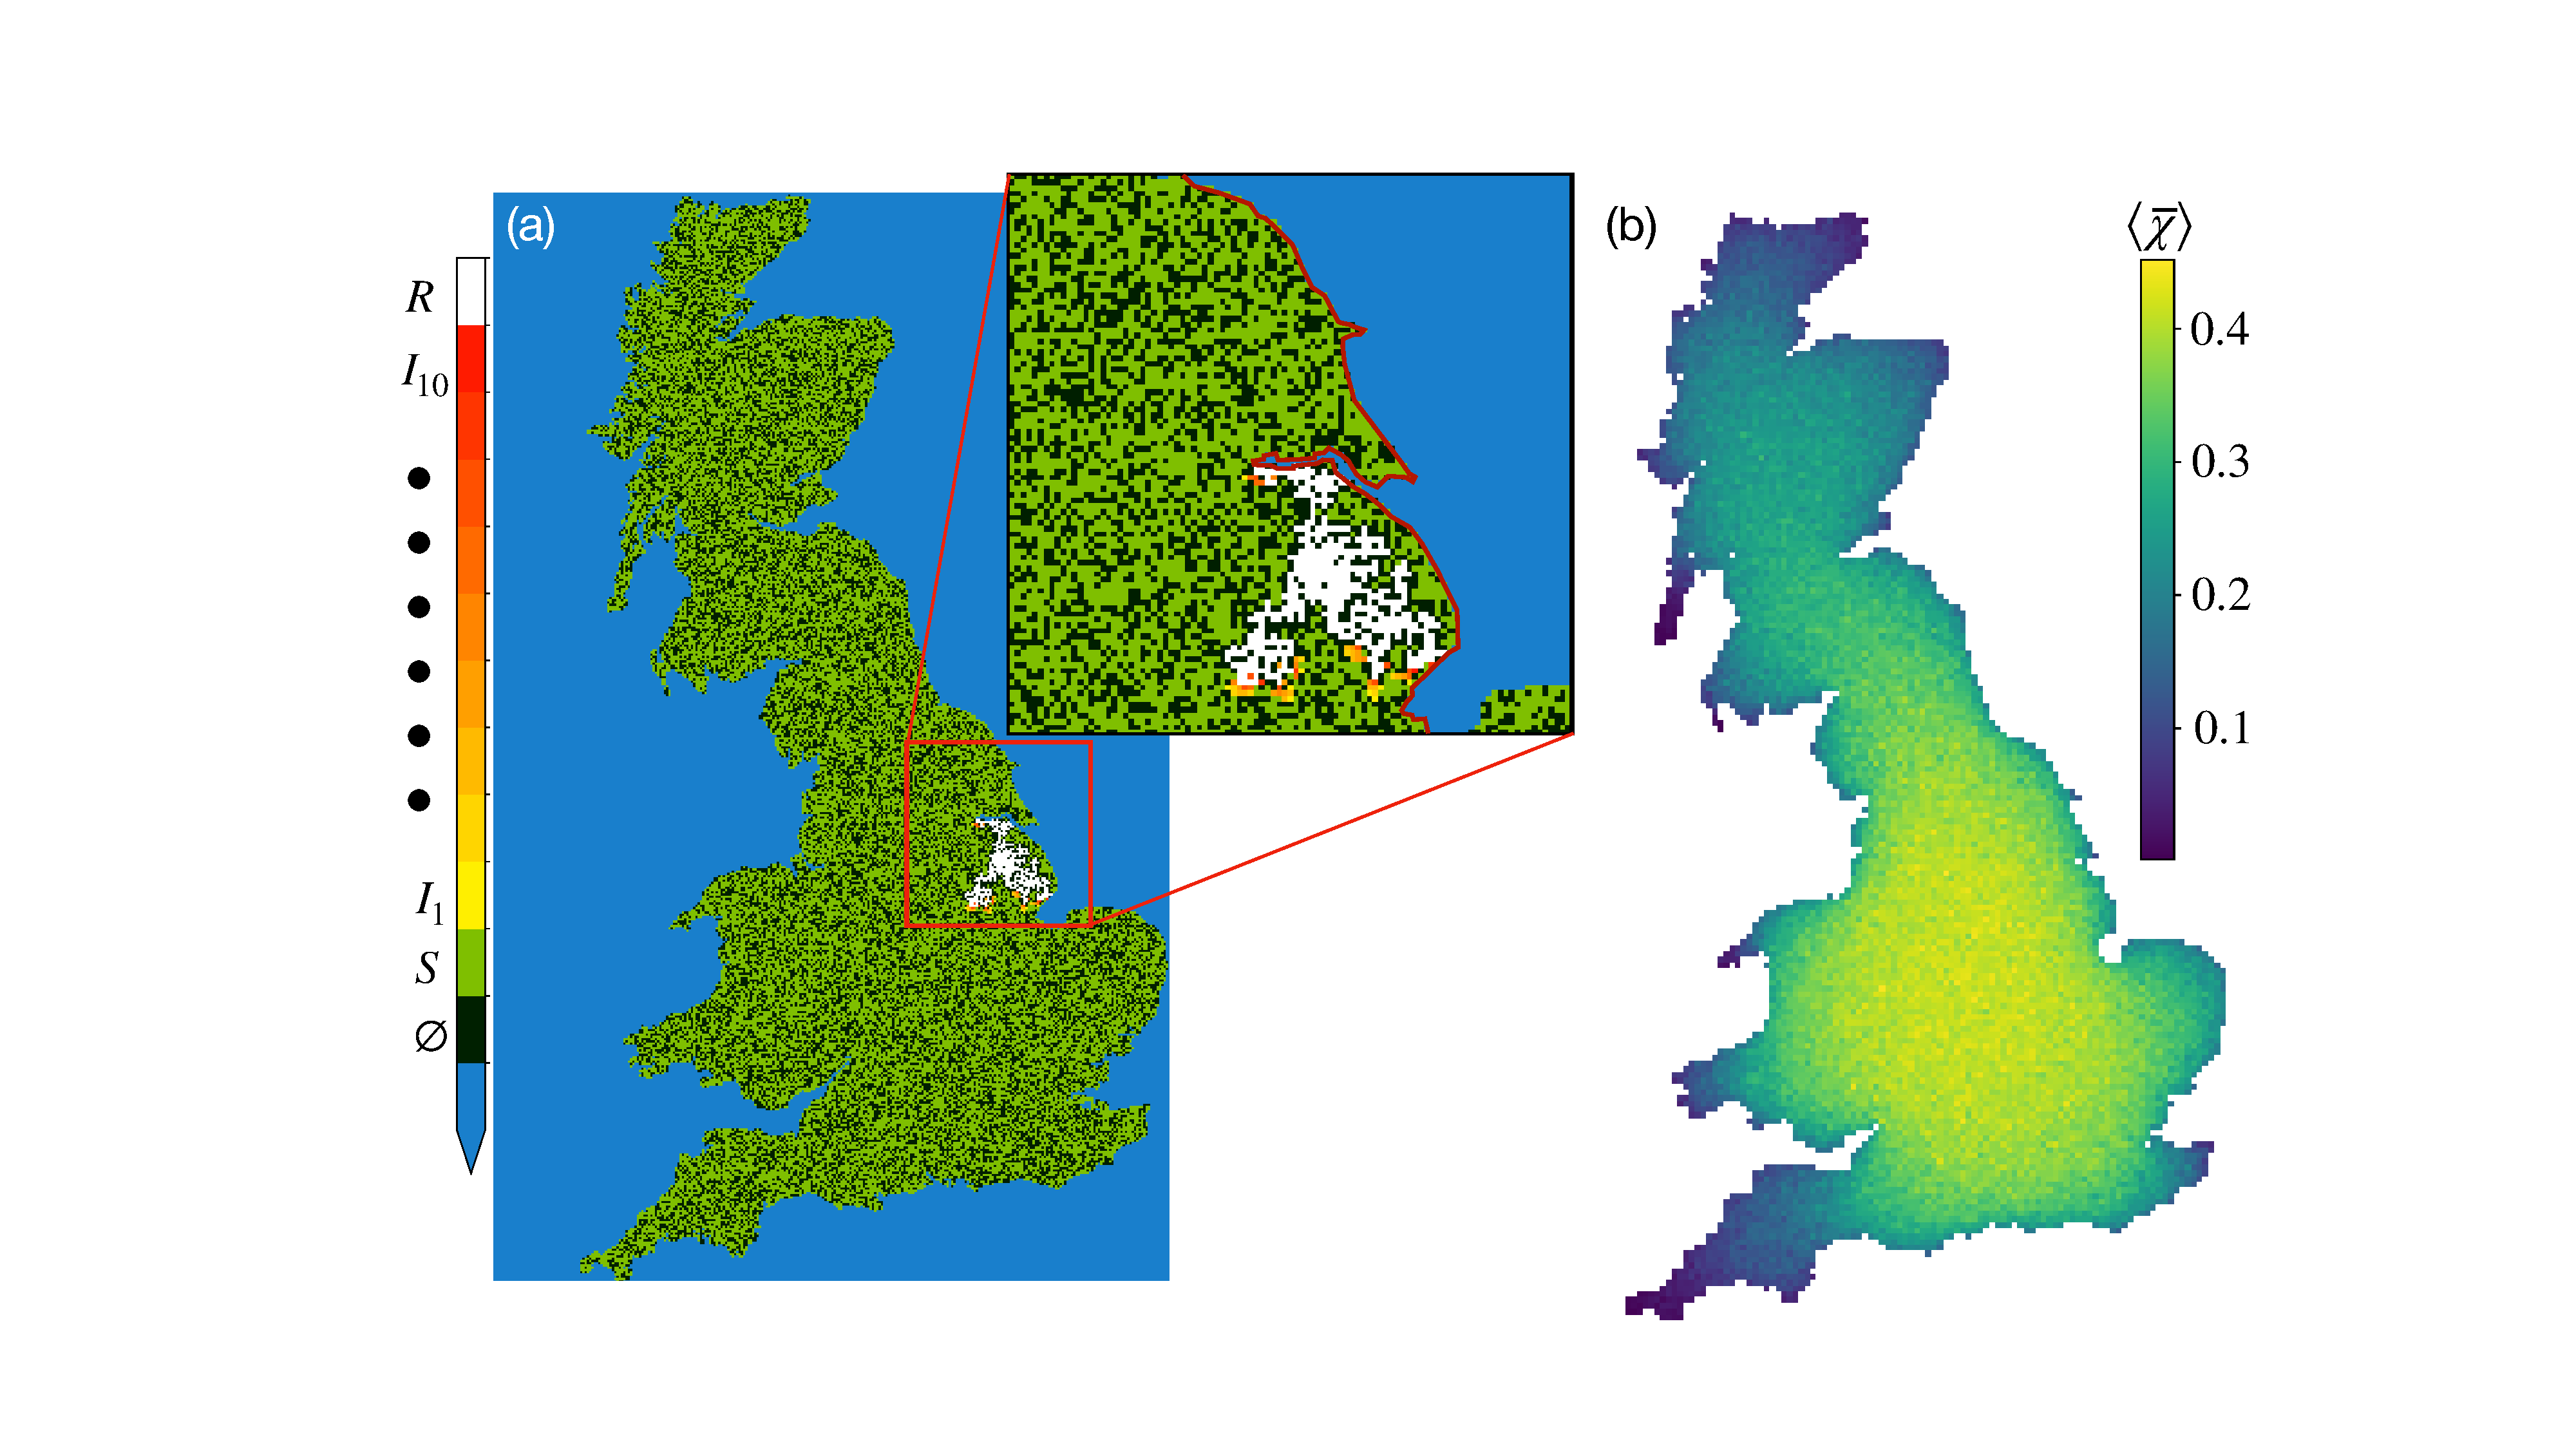
\includegraphics[scale=0.32]{chapter4/figures/figure1-GB-BCs.pdf}
    \caption{(a) The SLM spreading on a map of GB. The domain geometry and epicenter %
    location are non-trivial aspects likely to influence the spread of disease. The zoomed inset %
    shows an example of the Humber estuary preceding an infectious wave-front. 
    (b) Ensemble-averaged mortality-ratios are shown by colour for each spatial location with 
        parameters $\rho=0.65$ and $\beta=0.25$.}
    \label{fig:uk-spread-primer}
\end{figure}

In Figure \ref{fig:uk-spread-primer}(a), we see that coastline edge effects
might reduce the probability of an epidemic.
For example, epidemics emanating from epicentres located just below the 
Humber estuary (shown on the inset) could encounter more impedance when 
compared to more centrally-located positions.
Accordingly, SLM edge effects and domain BCs were examined by assessing the 
tree mortality from every possible epicentre, as shown in Figure \ref{fig:uk-spread-primer}(b).

Figure \ref{fig:uk-spread-primer}(b) reveals the ensemble-averaged mortality 
ratio, denoted by $\chi$.
The toy landscape-level SLM assumed parameter values just above threshold in a 2D square lattice,
where each simulation began from a single epicentre located at patch $(i, j)$.
Here, the mortality ratio captures the total epidemic impact, defined by: 
\begin{equation}
\label{eq:epi_impact}
    \chi=\frac{R_f}{S_0}
\end{equation}
where $R_f$ is the final number of patches in the removed state at $T_f$ and $S_0$ is the number of susceptible 
patches at time $T=0$.
Given the stochasticity, it is necessary to repeat simulations for each epicentre 
and calculate $\overline{\chi}$. Iterating over the whole of the GB in this way permits visualisation
of the spatial-susceptibility of the pathogen $\beta$, depicted by colour in Figure \ref{fig:uk-spread-primer}(b).

Figure \ref{fig:uk-spread-primer}(b) shows the result of the ensemble averaging $\chi$ for each
patch of land\footnote{Ensemble averages for each patch ($\approx 2 \times 10^5$ in total) was computationally costly. 
Hence, the domain resolution was coarse-grained to $\mathrm{5km \times 5km}$ sized-patches to reduce the number of simulations.
Even so, simulations were ensemble-averaged on the Leeds high-performance computing facility (ARC) using a task array.
The ensemble took approximately two hours on $25$ cores.}.
As expected, the domain BCs and map geometry change the resulting epidemic scale, 
mainly in Scotland and the south Eastern leg of GB towards Exeter and Plymouth.
Regardless, centralised regions show a roughly constant susceptibility. 
Higher epidemic parameters increased the mean mortality ratio and reduced spatial variations in the mortality ratio, whereas lowering epidemic parameters had the opposite effect.
Although Figure \ref{fig:uk-spread-primer}(b) paints an ideal epidemic scenario involving one infected patch at $t=0$,
we can assume an emerging epidemic within the SLM model depends non-trivially on the interplay of epicentre location and domain boundary.
 
 \newpage

\subsection{Realistic abundance data}

Figure \ref{fig:uk-oak-l.hill}(a) shows the distribution of oak in GB given by \cite{hill.data}.
The corresponding probability density function (\acrshort{pdf}) of canopy cover is shown in Figure \ref{fig:uk-oak-l.hill}(b).
Each pixel in Figure \ref{fig:uk-oak-l.hill}(a) depicts the predicted hectares
of oak canopy cover per kilometre squared of land, $\mathrm{ha/km^{2}}$, represented by colour. 
Therefore, each measure of abundance correlates to host density
(justified by the fact that $100\mathrm{ha} = 1 \mathrm{km^2}$), denoted by $\rho$.
The spatial map displays visual irregularities and population heterogeneity.

The PDF displayed in Figure \ref{fig:uk-oak-l.hill}(b) 
reveals that most land patches occupy lower canopy cover values.
Moreover, a small number ($\sim 5\%$) of high abundance values in the interval
$\rho \in [10, 35]\ \mathrm{ha/km^2}$ skewed the distribution; these high-valued density patches were reduced to $10\mathrm{ha/km^2}$, 
thereby capping the highest value to $10\%$ of oak canopy cover. 
The PDF describes a continuous distribution, which lies in contrast to the required binary-valued distribution of hosts 
within the SLM. Accordingly, we introduce a threshold function to navigate the problem:  
\begin{equation}
  \phi(\rho) =
  \begin{cases}
    1 & \rho_{i,j}\geq\rho \\
    0 & \rho_{i,j}<\rho
  \end{cases}
\end{equation}
where the canopy cover $\rho\in[0, 10]\ \mathrm{ha/km^{2}}$ acts as a threshold value, 
above which, all patches become susceptible and assumes the numerical value of unity (i.e. $\rho < \rho_{i,j} = 1$).
Conversely, insusceptible states are described when $\rho \geq \rho_{i,j}= 0$.
The inset of Figure \ref{fig:uk-oak-l.hill}(b) visually depicts the abundance threshold function; 
the vertical black line is an arbitrary threshold $\rho$, and all canopy cover values less and greater than
$\rho$ describe insusceptible and susceptible, respectively.
Susceptible patches have enough hosts to support disease survival, growth, and spread in this interpretation. %
Patches of land below the abundance threshold are presumed insusceptible on account of insufficient hosts.

\newpage

\begin{figure}
    \centering
    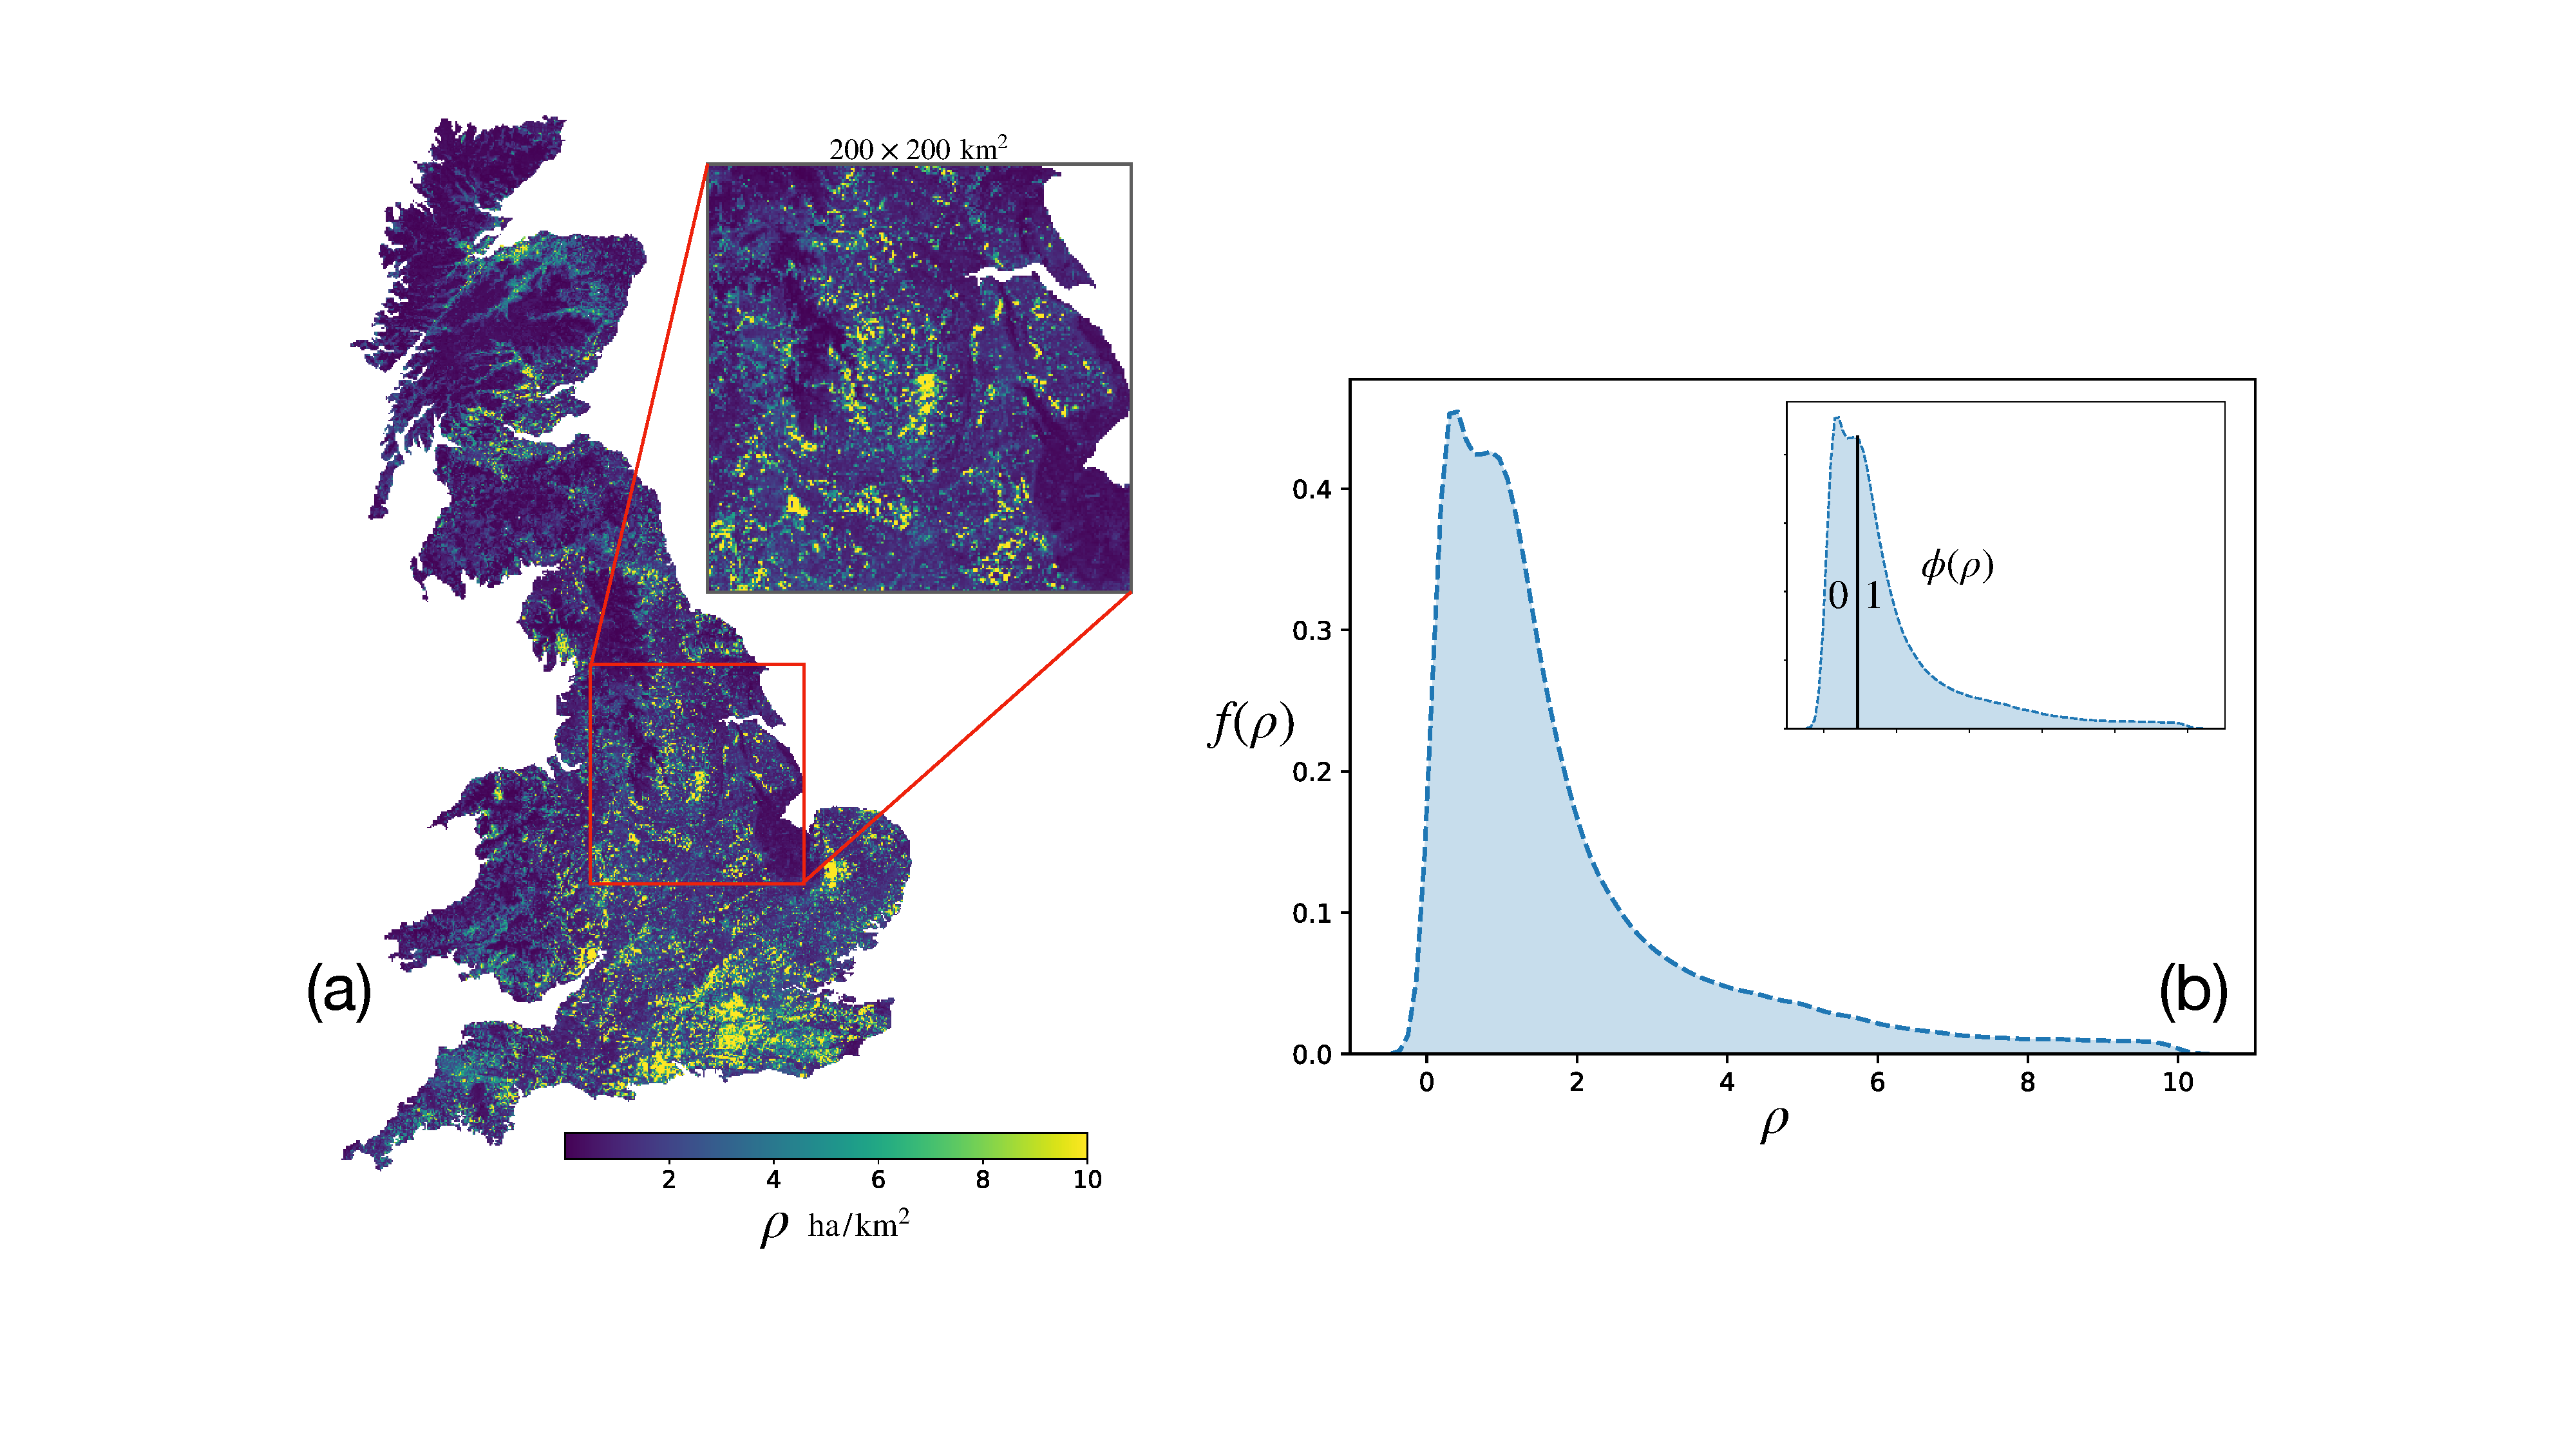
\includegraphics[scale=0.32]{chapter4/figures/figure3.pdf}
    \caption{
    (a) The abundance distribution of common oak (\textit{Quercus robur}) given by \cite{hill.data}. Each pixel describes a predicted value of abundance with units hectares of canopy cover per kilometer squared of land ($\mathrm{ha/km^2}$). 
    (b) The probability density function of oak abundance in GB, $f(\rho)\ \mathrm{ha/km^2}$. 
    The zoomed inset illustrates the process of generating threshold function $\phi$.}
    \label{fig:uk-oak-l.hill}
\end{figure}

Earlier in Chapter \ref{chapter:SLM}, hosts distributions were easily characterised by $\rho \in [0, 1]$, 
describing a uniform density throughout a square lattice.
Now, however, host heterogeneity prevents a simple description of density.
Nevertheless, by considering the percentage of susceptible patches,
one can define effective landscape density $\rho^*$:
\begin{equation}
    \label{eq:rho_eff}
  \rho^{*} = \frac{\sum^{i, j} ( \rho_{i,j} \geq \rho )}{|\mathcal{L}_{GB}|}
\end{equation}
where $\mathcal{L}_{GB}$ represents host distribution over Great Britain. 
The terms $\sum^{i, j} (\rho_{i,j} \geq \rho)$ and $|\mathcal{L}_{GB}|$ represent 
the total number of susceptible patches and total landmass respectively. 
Given an increase in the threshold $\rho$, the effective density $\rho^*$ decreases; 
likewise, a decrease in $\rho$ increases $\rho^*$ as more patches become susceptible. 
Thus, $\rho^{*}$ presents a convenient, although crude, agent
to adjust the host distribution to higher or lower densities.

\subsection{Epidemics through heterogeneous landscapes}

Applying the effective density ($\rho^{*}$) of Equation \ref{eq:rho_eff},
we can initialise a set of binary-valued SLM heterogeneous domains. 
Figure \ref{fig:ch4_uk_spread} shows three variations of effective density
$\rho^{*} \in [0.40, 0.50, 0.60]$, alongside the corresponding thresholds of
abundance canopy cover shown below. In Figure \ref{fig:ch4_uk_spread}, the SLM
is simulated with infectiviy $\beta=0.25$, until pathogen extinction, 
shown through through four time-steps. Between panels (a) (e) and (i), 
the differences in the domain density are visible,
as larger values of abundance thresholds produce lower density maps.
For the three simulations shown in Figure \ref{fig:ch4_uk_spread}, 
epicentres were placed in the south, where the canopy cover is most dense. 

Previously, density was uniform in all directions, 
but now heterogeneity unevenly distributes susceptible hosts. 
Notwithstanding, we may still expect an epidemic to emerge if density 
and infectivity parameters satisfy a critical threshold, as explored in Chapter \ref{chapter:SLM}.
For all $\rho^*$ values shown in Figure \ref{fig:oak-spatial-ensemble}, 
initial outbreaks ($0<t<250$) spread above the threshold.
Although at $\rho^*=0.40$, we notice a significant drop in disease progression 
beyond $t=250$ in (c-d), approximately extending from Oxford to Buckinghamshire due to a low density;
in contrast, $\rho^*=0.50$ and $\rho^*=0.60$ spread above the threshold for all panels.

In Figure \ref{fig:ch4_uk_spread} we can observe a spatial dependence in the SLM threshold,
where above-threshold regions (e.g. the in south) depend on the host density $\rho^*$ parameter.
In particular, Figure \ref{fig:ch4_uk_spread} demonstrates that increasing $\rho^*$ can lead to channels opening between different above-threshold regions, thus permitting disease to invade new regions\textemdash i.e. compare Figure \ref{fig:ch4_uk_spread}(d), (h), and (l), where only higher density simulations spread progressively further North.

Unfortunately, the definition of percolation (as per Equation \ref{eq:critical_threshold_1d}) becomes obscure in light of the irregular domain configuration shown in 
Figure \ref{fig:oak-spatial-ensemble}, primarily because the extent between borders is now non-uniform
and dependant on epicentre location.
Furthermore, simulation time series are subject to additional noise on account of heterogeneity, 
making velocity-based metrics (as shown in Equation \ref{eq:vel_eff_r}) hard to use. 
Subsequently, the examination of disease progression will focus on the mortality ratio $\chi$, 
as its measurement depends only on the final value of removed trees.

\begin{figure}
    \centering
    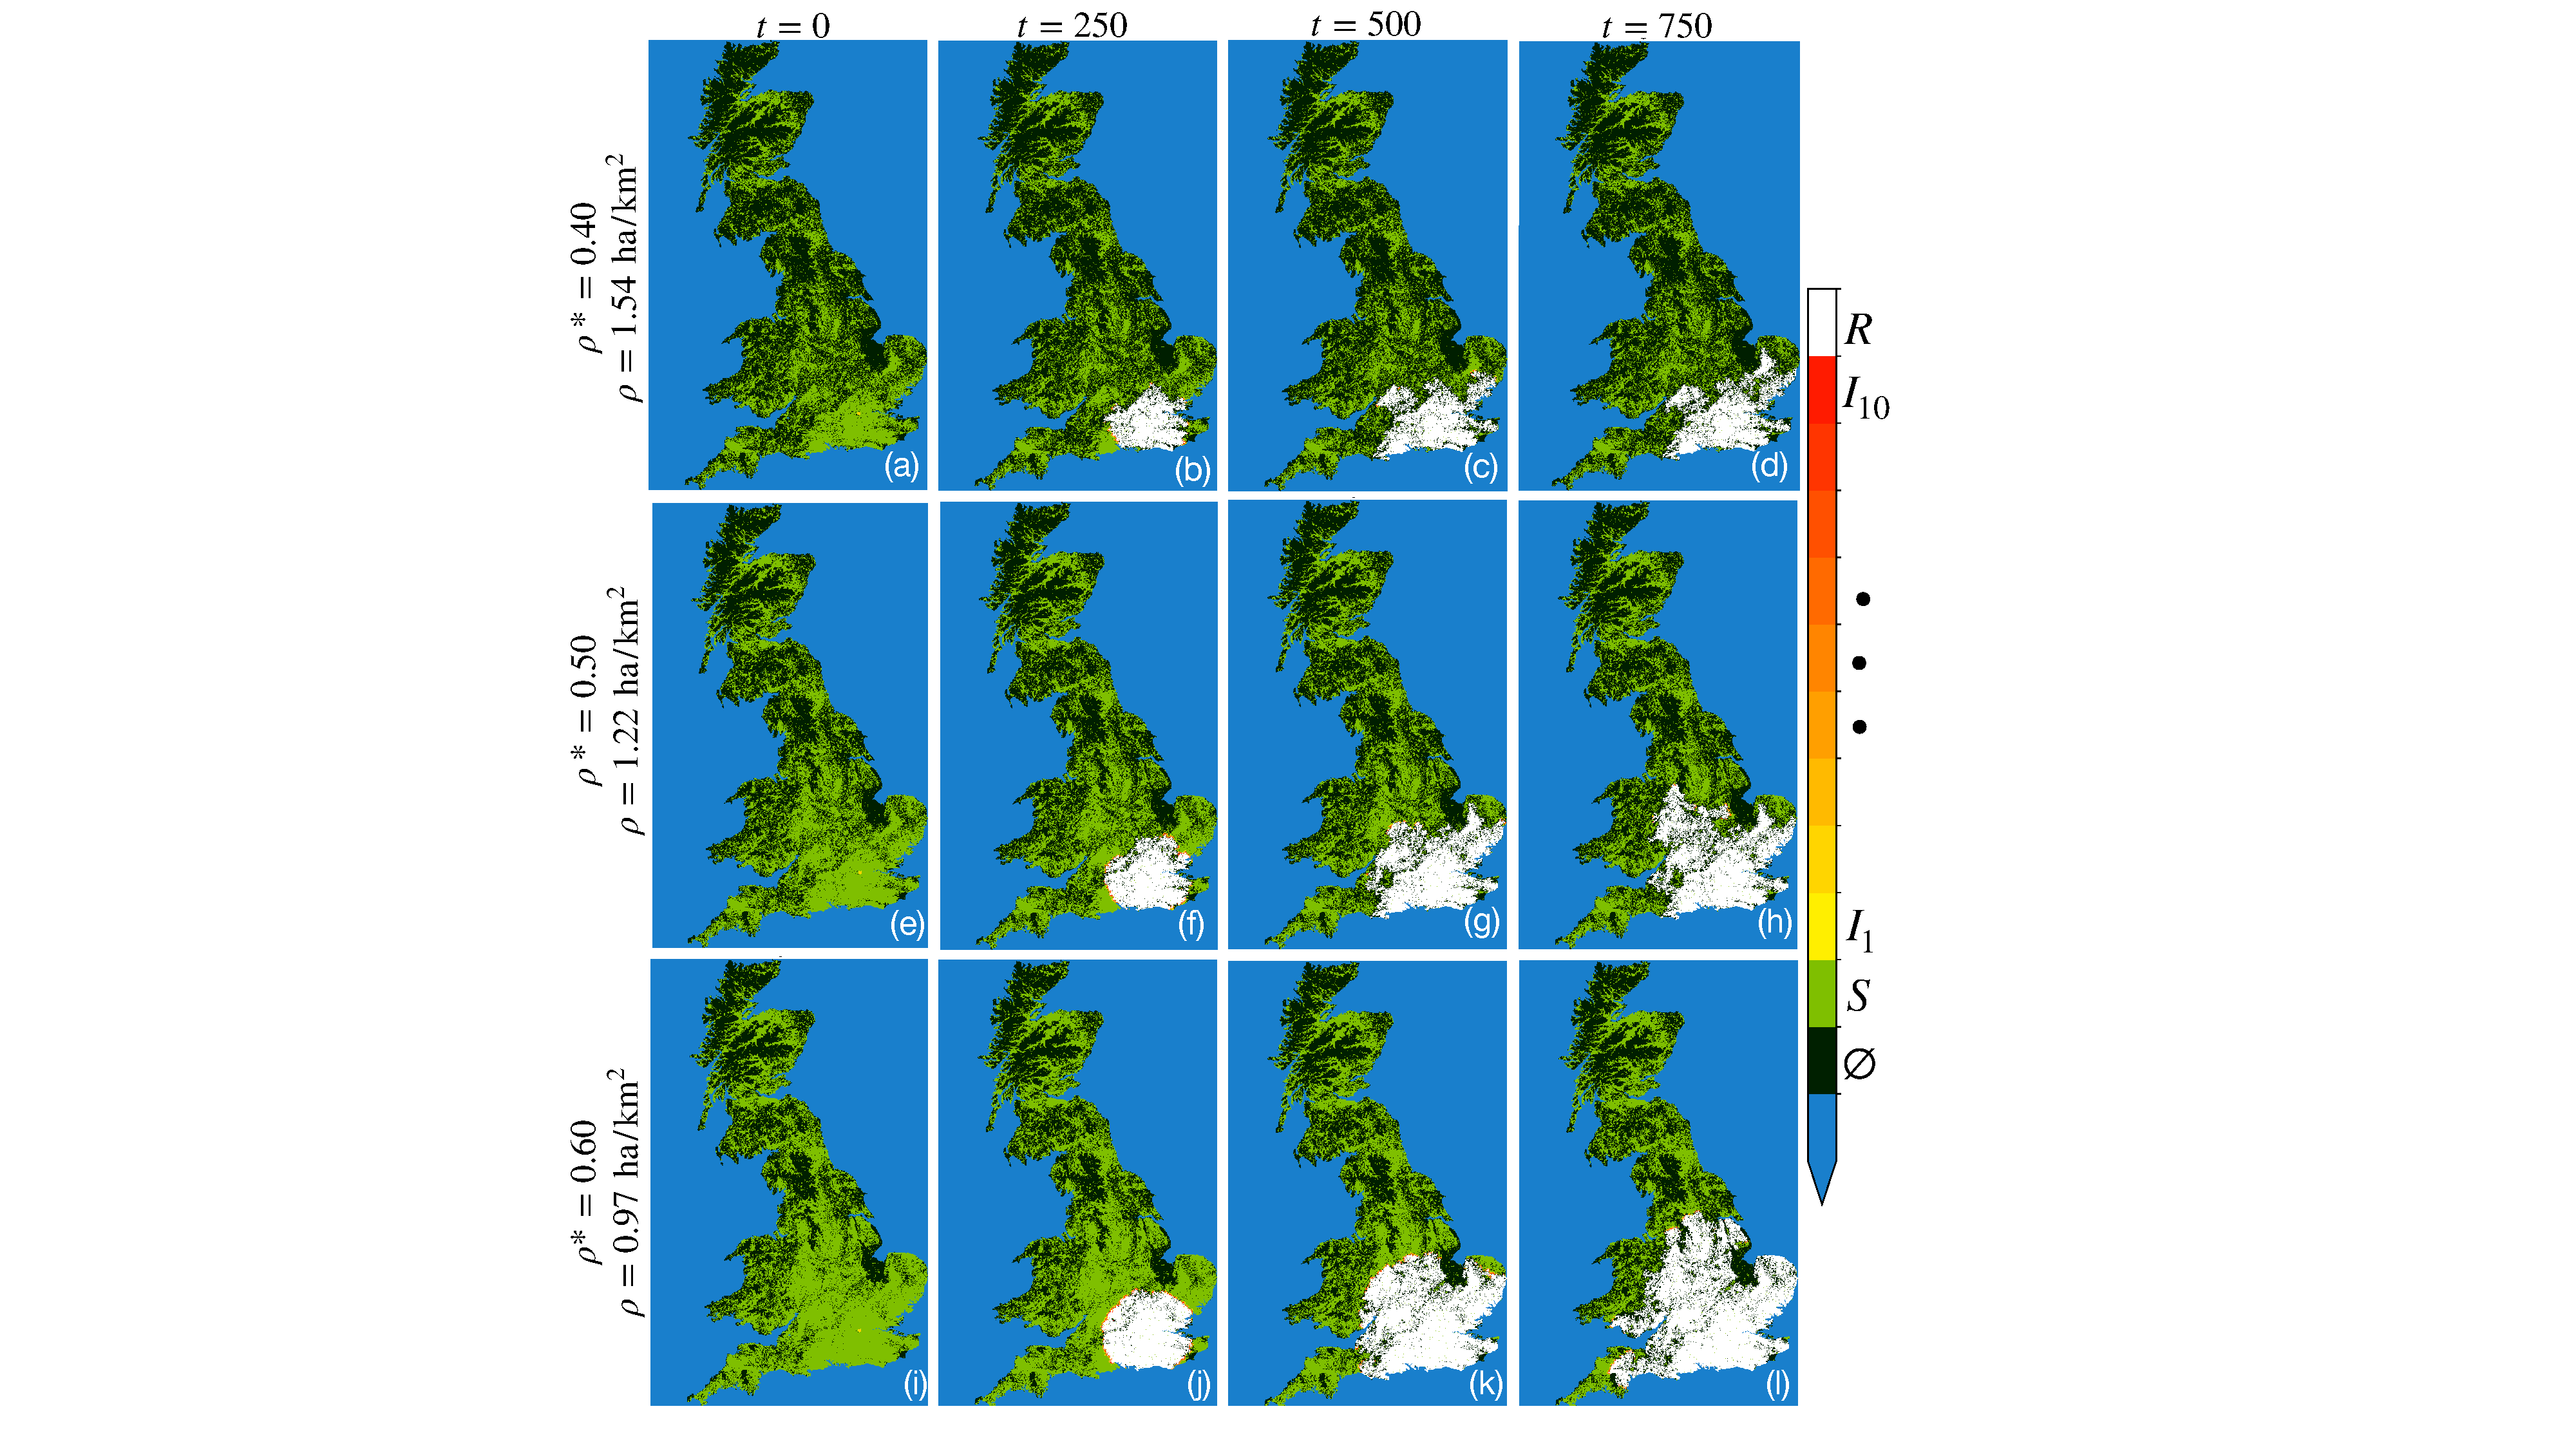
\includegraphics[scale=0.490]{chapter4/figures/figure4.pdf}
    \caption{The simple lattice model running on a binary-valued Oak domain with infectivity $\beta=0.25$ for three variations of effective density $\rho^*$.}
    \label{fig:ch4_uk_spread}
\end{figure}

\subsection{Spatially dependent ensembles}
\label{sec:slm-spatial-ensembles}

The observations of spatially varying thresholds, as revealed by Figure \ref{fig:ch4_uk_spread}, 
motivates an examination of epidemic impact as a function of epicentre location.
As such, we apply the same ensemble averaging method discussed previously (in Figure \ref{fig:uk-spread-primer})
to the oak abundance data set. That is, treating each location $(i,j)$ in GB as a potential
epicentre and ensemble averaging host mortality over replicate simulations.
Here, the mortality ratio $\big\langle \overline{\chi} \big\rangle \in [0, 1]$ describes the ratio 
of removed host patches to the total number of susceptible patches at $t=0$ and 
expresses the final sized epidemic in the SLM. 

The result of spatial ensemble averages are shown in Figure \ref{fig:oak-spatial-ensemble}
for three different effective densities and one value of infectivity $\beta=0.25$. 
The values of effective density in Figure \ref{fig:oak-spatial-ensemble} are arbitrary,
but crucially exhibit the heterogeneous SLM behaviour. Unsurprisingly, increasing the effective density yields a 
higher mortality ratio (as defined by Equation \ref{eq:epi_impact}).
In turn, a higher mortality increases the magnitude of colour bars in Figures \ref{fig:oak-spatial-ensemble}(a-c). Alongside a more severe mortality ratio, a higher $\rho^*$
value also permits disease propagation over more extensive regions, witnessed by comparing Figures \ref{fig:oak-spatial-ensemble}(a) and (c).

In Figures \ref{fig:oak-spatial-ensemble}(a-c), yellow regions highlight where the pathogen is most 
likely to spread through susceptible hosts. In the toy model, mortality is approximately independent of epicentre location, 
provided sufficient (Von Neumann) connectivity between patches, supported by uniform yellow contours within susceptible regions.
In panel (a), the spatial locations encircled in dashed red highlight a region of instability that appears to separate two susceptible regions.
In these regions, the epidemic impact could vary significantly, 
consequently prompting the corresponding plots of mortality variance in Figures \ref{fig:oak-spatial-ensemble}(d-f).

\begin{figure}
    \centering
    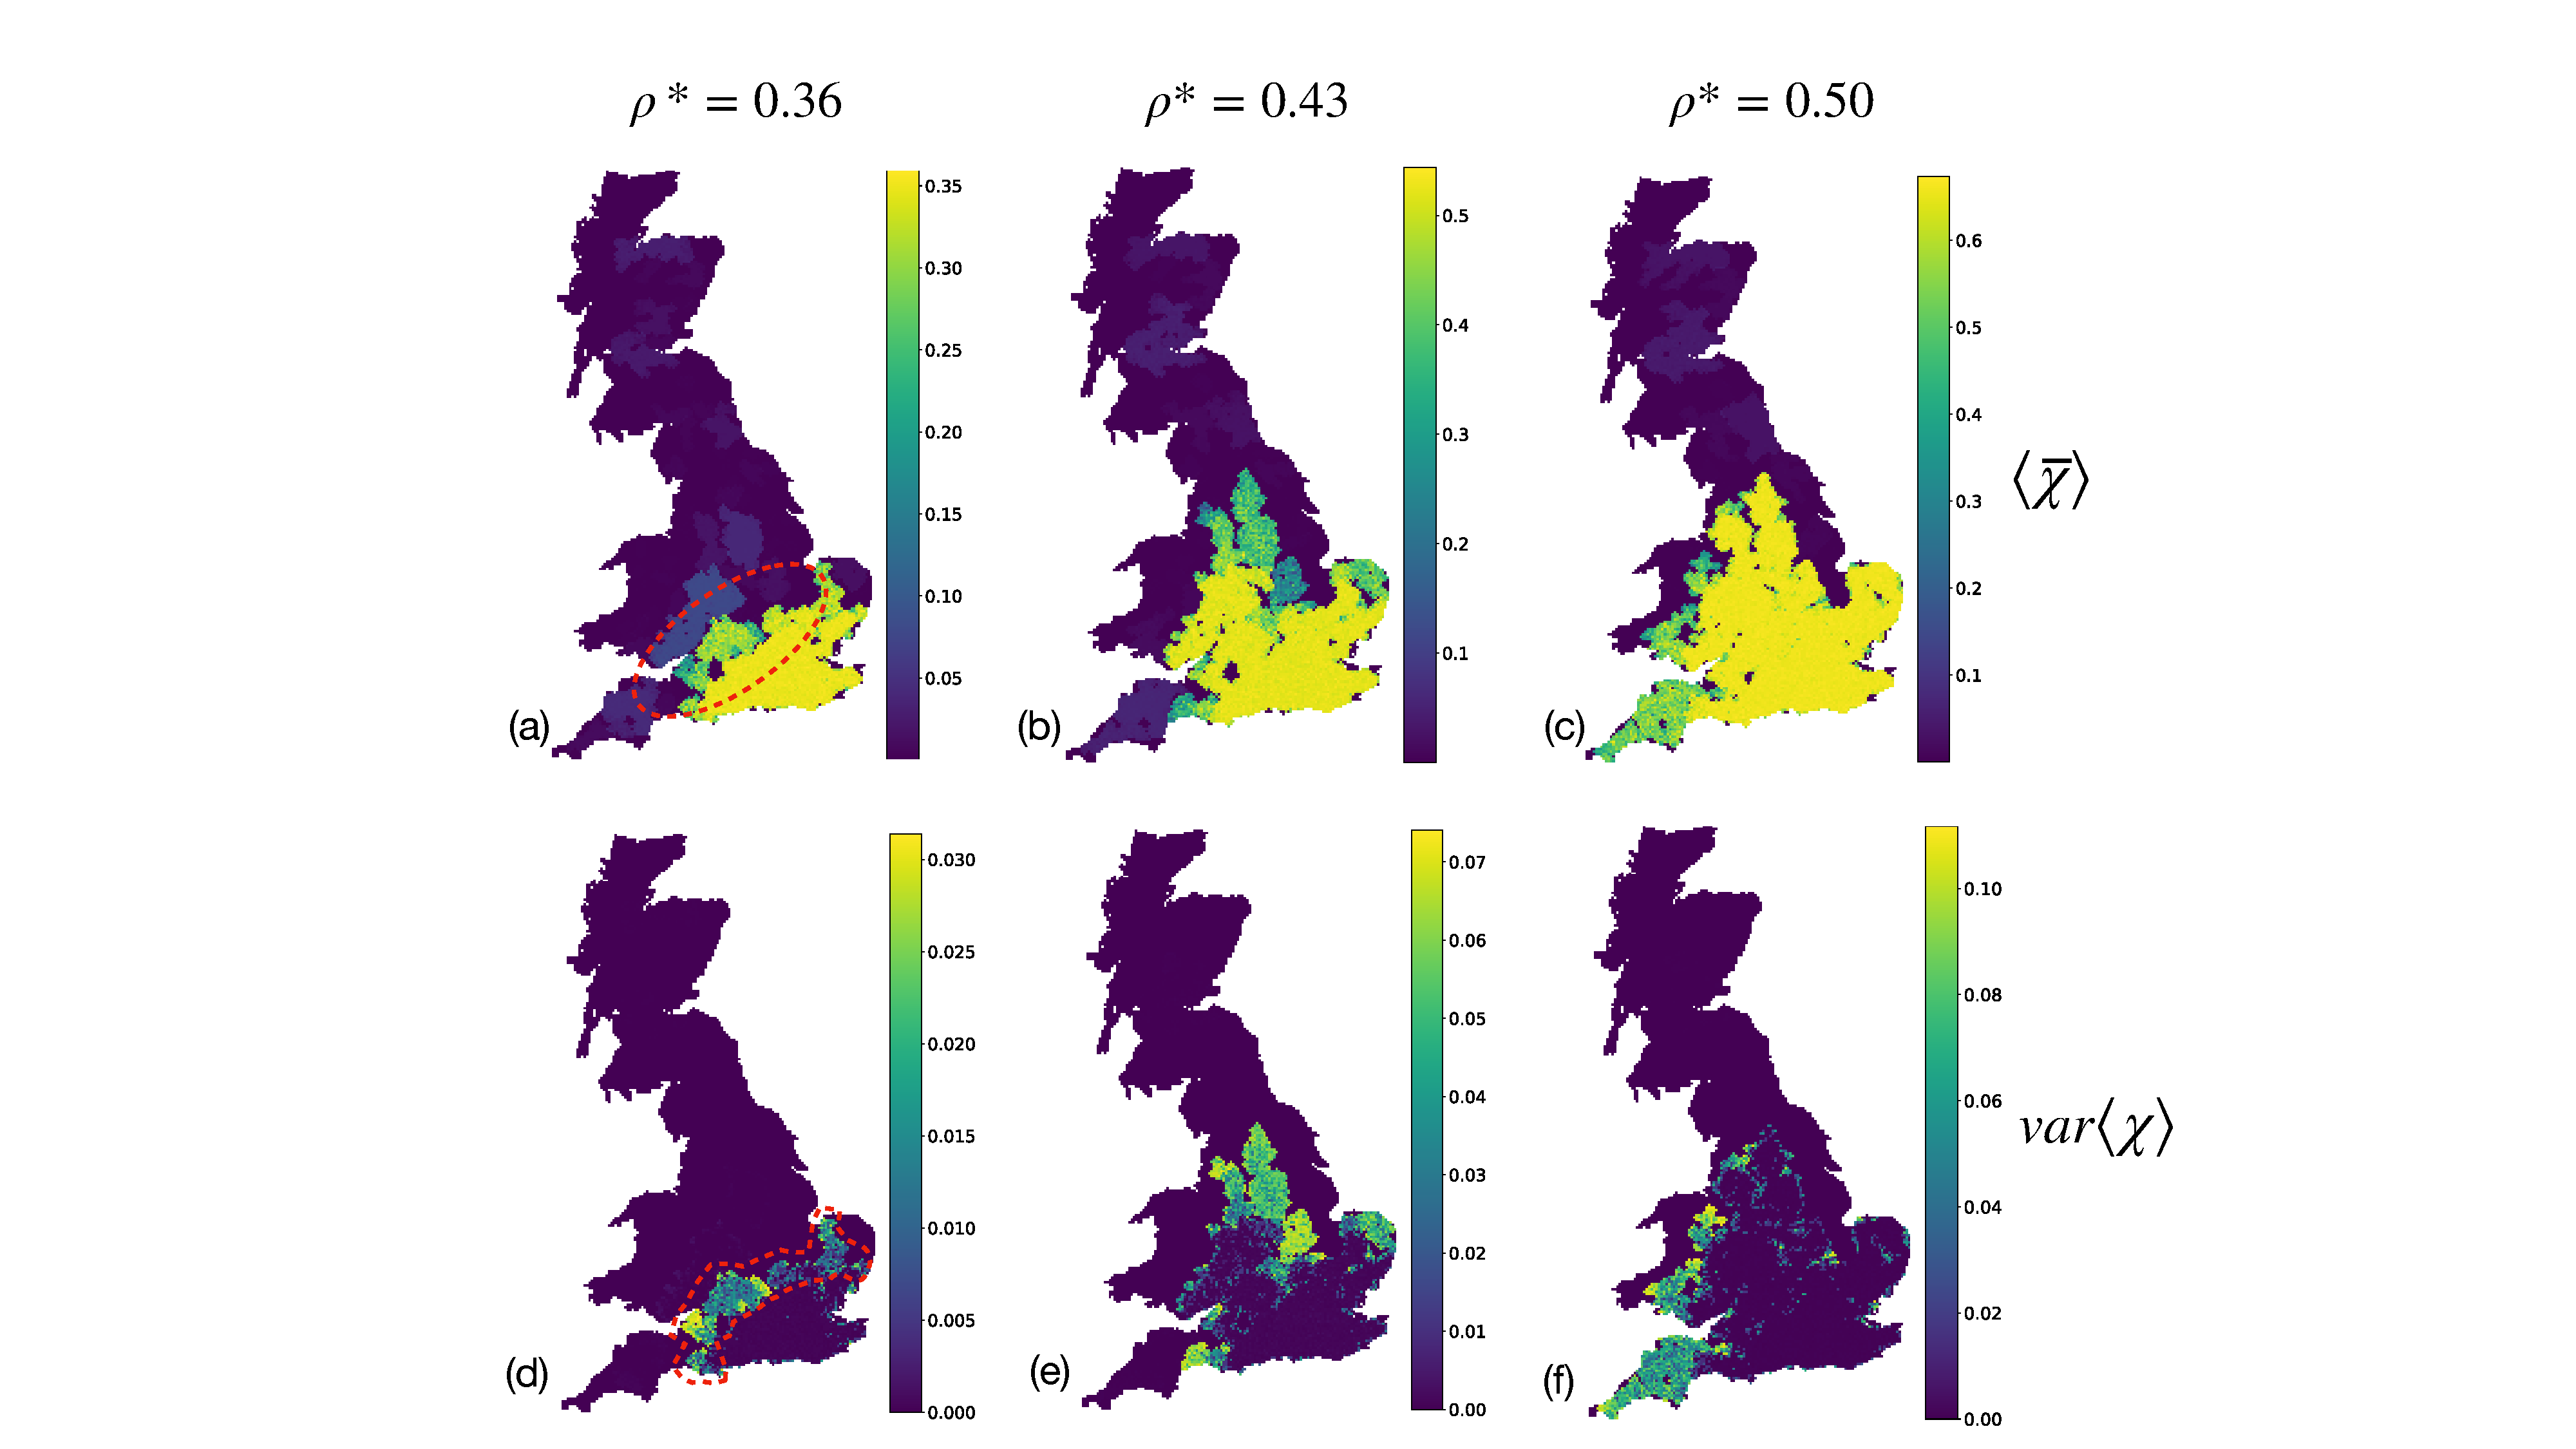
\includegraphics[scale=0.4]{chapter4/figures/figure5.pdf}
    \caption{Spatial phase showing ensemble statistics over the oak data-set for three variations of density threshold $\phi(\rho): \rho \in [0.37, 0.43, 0.50]$ and fixed infectivity $\beta=0.25$. (a-c) The ensemble mean of mortality ratio $\chi$ measured for each pixel epicenter. The dotted red circle in Fig (a) shows two neighbouring susceptible regions. (d-f) Ensemble variance over $\chi$. The dotted shape in (d) highlights an unstable region of high variance and uncertainty separating two susceptible areas of the population in Fig (a).}
    \label{fig:oak-spatial-ensemble}
\end{figure}

Mapping the ensemble averaged mortality variance reveals uncertainty, where regions support the possibility of both epidemic and extinction.
Figure \ref{fig:oak-spatial-ensemble}(d) captures a region of uncertainty, highlighted in red.
In this region, the toy model may or may not give rise to a large scale epidemic, as opposed to the most southerly, 
high-mortality region beneath the dashed red lines. Panels (e) and (f) show a variance only in the edges of the centrally
located susceptible region. It is alluring to consider the implications of high variance regions in Figures \ref{fig:oak-spatial-ensemble}(d-f)
in the context of epidemic control. Namely, we may suppose that epidemic control through high variance regions could be an effective strategy
in stopping the spread of disease.
Although the mortality ratio ($\chi$) categorises the overall epidemic scale in the SLM, 
it fails to reflect any information about how far an epidemic is likely to propagate.
Recording the maximum distance travelled by the pathogen proved a helpful method to illustrate spatial progression,
maps of `maximum distance' are displayed in appendix \ref{a:landscape-toy-model}. 


\subsection{Heterogeneous parameter sweeps}

Thus far, spatial ensemble analysis rests on a fixed infectivity ($\beta=0.25$)
and has focused on mapping mortality with a varying effective density parameter $\rho^*$.
In this section, we investigate the entire parameter space of $\rho^*$ and $\beta$.
Figure \ref{fig:heterogeneous-phase-space} depicts a full parameter sweep of the toy landscape SLM.
Due to more host units in computer memory, simulating the spread of disease in the toy landscape SLM is more 
computationally challenging when compared to the ideal square SLM in Chapter \ref{ch3:two-param-model}.
Even though epidemics in the toy SLM are conditioned on epicentre location (confirmed in section \ref{sec:slm-spatial-ensembles}),
analysing a single epicentre is sufficient to capture the essential toy model behaviour.
Ergo, we present an analysis through a single epicentre.

Figure \ref{fig:heterogeneous-phase-space} shows the ensemble-averaged epidemic phase space of the toy landscape SLM
through a epicentre\textemdash indicated by the red point in Figure \ref{fig:heterogeneous-phase-space}(a).
The Parameter sweeps of $\rho^{*}$ and $\beta$ demonstrate multiple discontinuities and sharp increases in $\chi$
for particular combinations of $\rho^{*}$ and $\beta$; this contrast with the parameter sweeps inside a homogeneous square domain.
Moreover, Figure \ref{fig:heterogeneous-phase-space}(b) reveals a large asymmetry between $\rho^*$ and $\beta$ 
as more discontinuous jumps appear most when $\rho^*$ is increased, i.e. moving horizontally 
through Figure \ref{fig:heterogeneous-phase-space}(b). Hence, host heterogeneity gives rise to distinct behaviours for both
$\rho^*$ and $\beta$ axes, as opposed to the (approximately) symmetric ensembles in a homogeneous square domain.  

Figures \ref{fig:heterogeneous-phase-space}(c-d) contrast behavioural differences between 
$\rho^*$ and $\beta$ axes. Specifically, we compare one-dimensional slices through both parameters $\rho^*$ and $\beta$.
Figure \ref{fig:heterogeneous-phase-space}(d) details how variations of $\rho^*$ effect the model behaviour through $\beta$-space. 
Interestingly, Figure \ref{fig:heterogeneous-phase-space}(d) depicts the same infectivity threshold of $\beta\sim 0.10$, 
identical to the SLM evolving on a uniform square domain. When $\beta$ increases, fewer discontinuities arise when
compared to $\rho^*$, as evidenced by smoother curves. 

For each value of density in Figure \ref{fig:heterogeneous-phase-space}(d), 
the mortality remains fixed beyond $\beta \sim 0.30$.
We can understand the independence between $\chi$ and infectivity through a numerical example:
the probability of a susceptible patch remaining susceptible when it encounters 
an infected neighbour is given by Equation \ref{eq:pr_s_s} as $Pr(S \rightarrow S) = (1 - 0.30)^{10} = 0.03$. 
Therefore, on average the pathogen transmits successfully to susceptible neighbours with probability $Pr(S\rightarrow I)=0.97$, 
e.g. if a particular epicentre belongs to a susceptible region containing $100$ patches, only three patches remain susceptible. 
In this instance, most patches in the cluster become infected, and further increases in $\beta$ do not affect the 
mortality\footnote{
Increasing the infectivity to $\beta=0.40$ yields a $Pr(S \rightarrow S) = 0.006$, 
leading to negligible changes in the final epidemic size\textemdash however, the rate of progression is still faster.
}. 
When $\beta \sim 0.30 $, only increases to the domain density have the potential to raise the final epidemic size, 
indicated by the increases in the height of the curves in Figure \ref{fig:heterogeneous-phase-space}(d). 

\begin{figure}
    \centering
    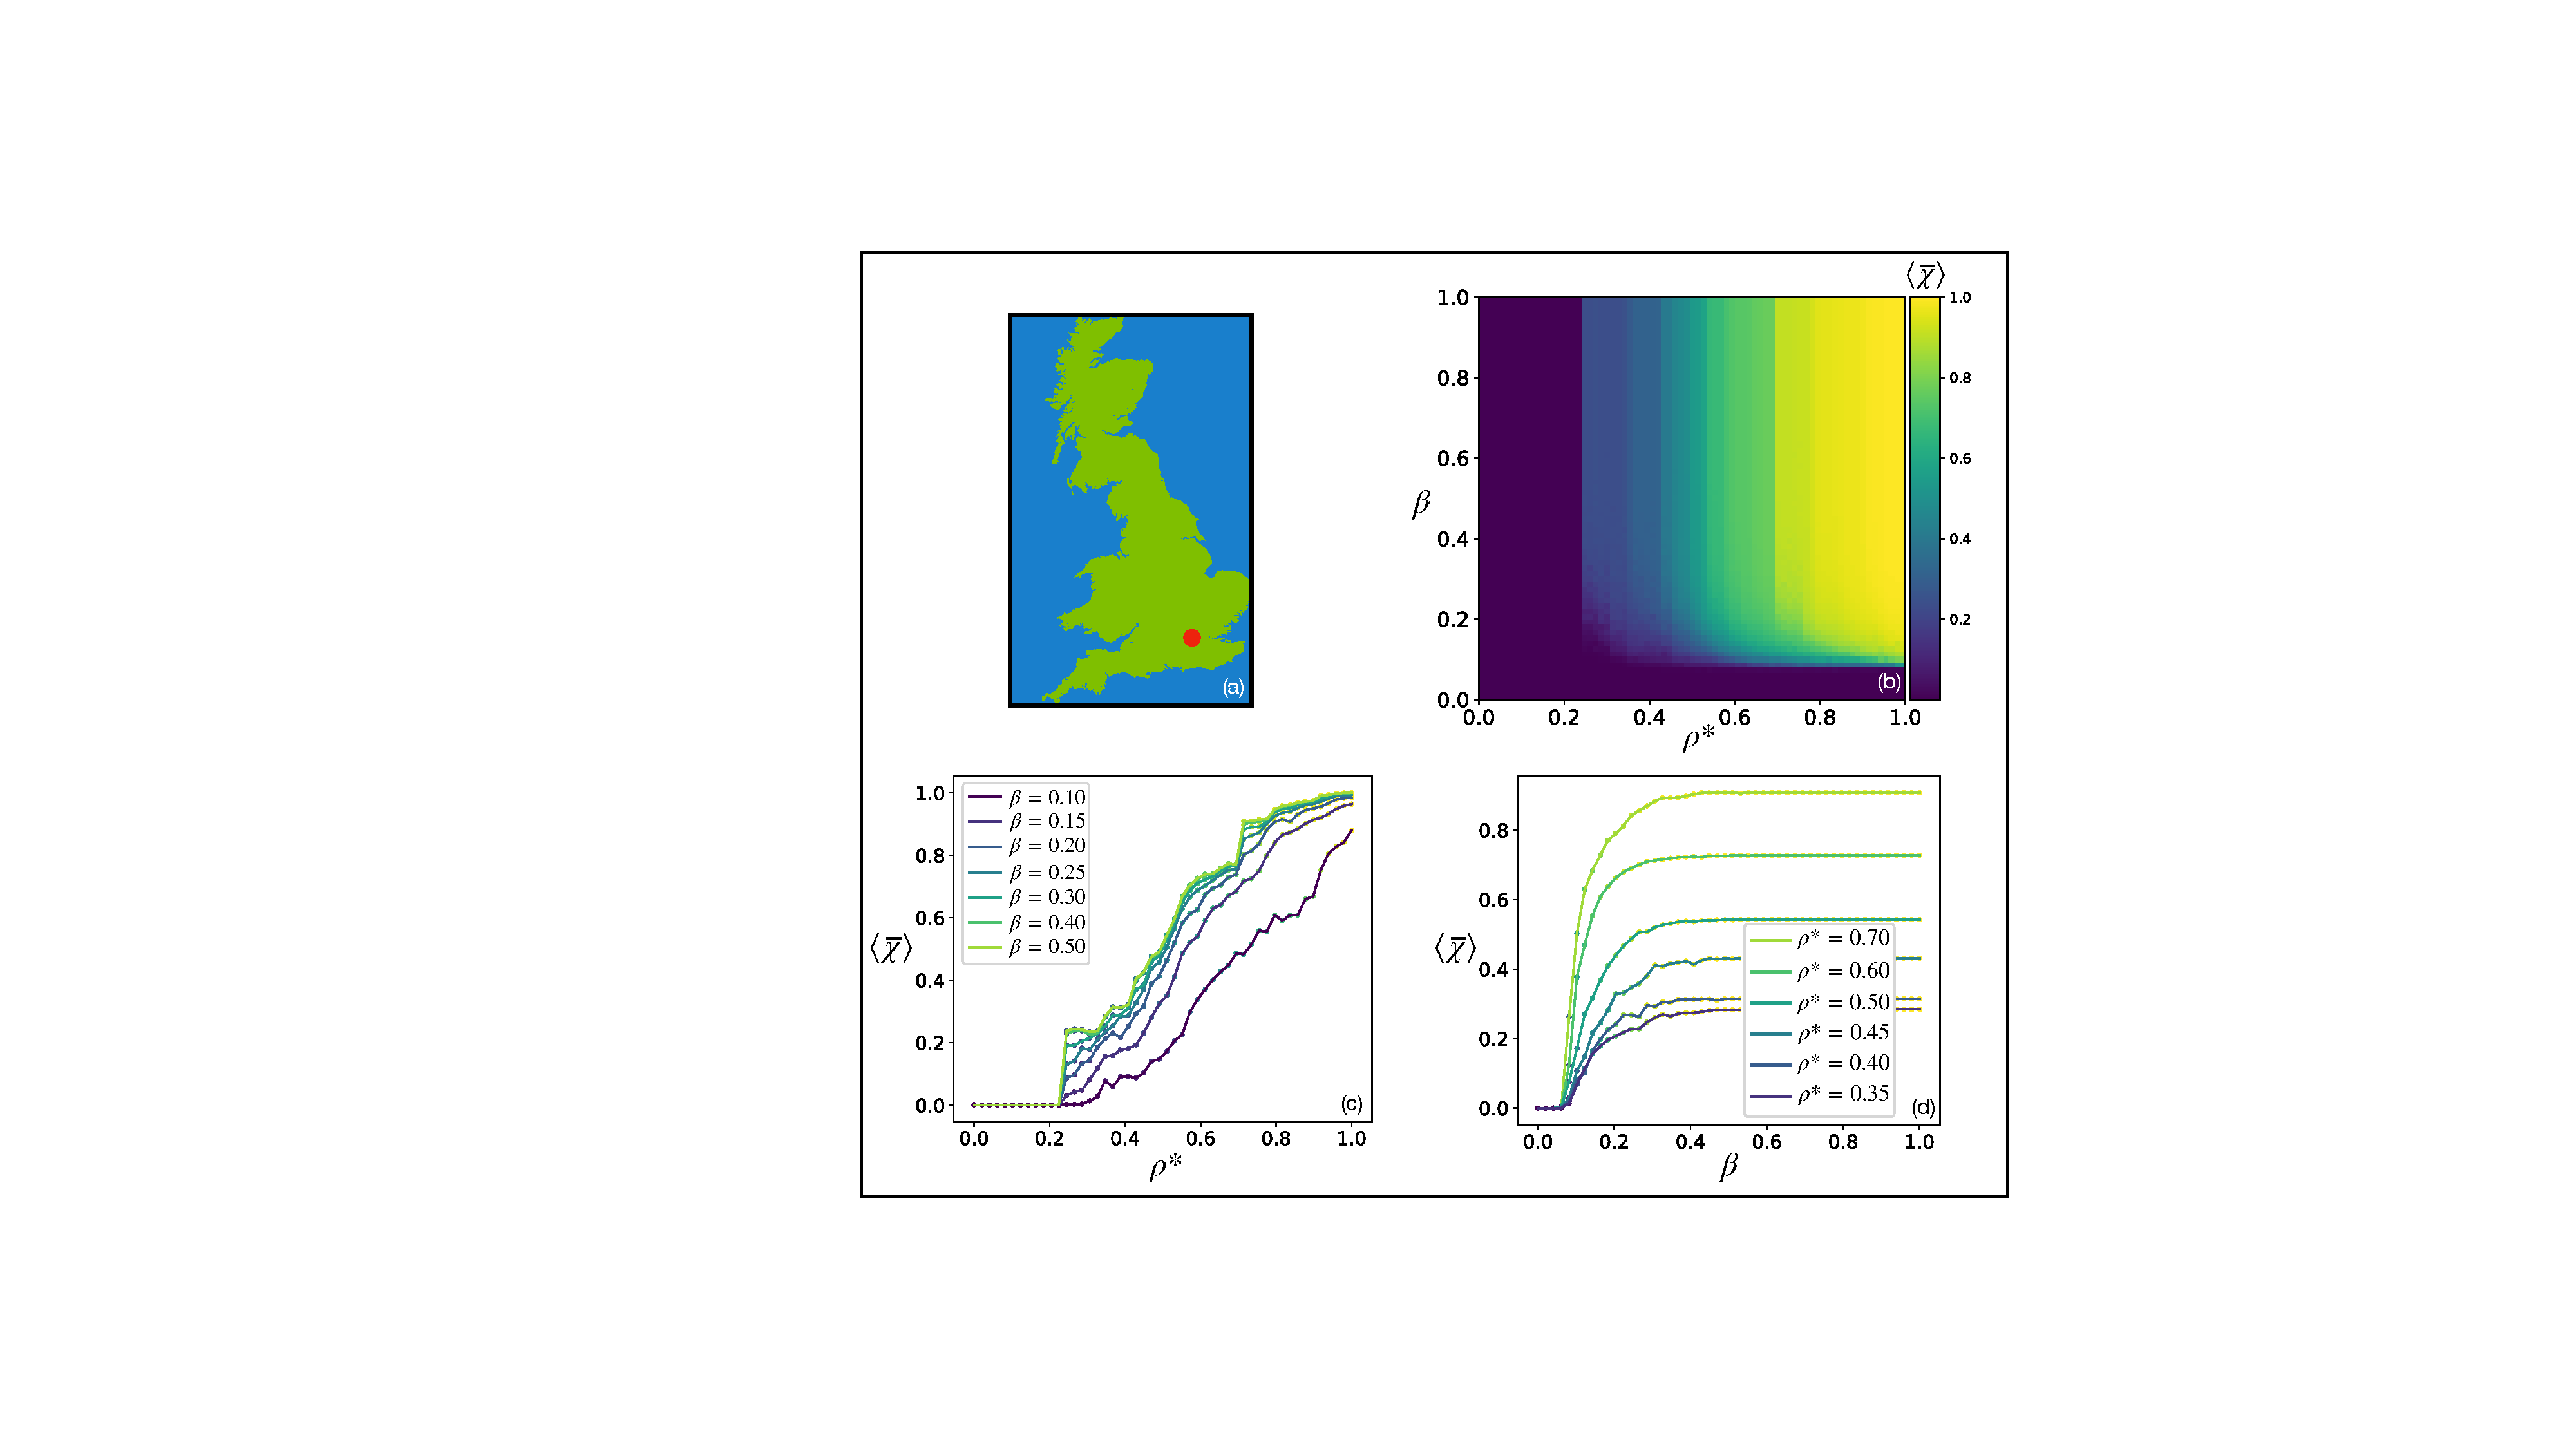
\includegraphics[scale=0.55]{chapter4/figures/figure4-param-sweeps.pdf}
    \caption{
    The result of beginning from a single fixed epicentre (shown in red inside panel (a)),
    ensemble-averaged parameter sweeps of the toy model display a threshold-like behaviour.
    (b) The mortality ratio is plotted over the two-dimensional parameter space of $\rho^*$ and $\beta$. 
    (c) A one-dimensional plot of mortality as a function of host density is shown alongside several slices of infectivity, indicated by colour.
    (d) The mortality ratio is found over infectivity $\beta$ for different values of effective density $\rho^{*}$.
    }
    \label{fig:heterogeneous-phase-space}
\end{figure}

\newpage

\section{Discussion}
\label{sec:ch4-discussion}

In this Chapter, we explored two applications of the SLM viz; early warning signals and a toy landscape-level model.
The original analysis conducted by \cite{OROZCOFUENTES201912} relied on a velocity metric based on the number of 
infected and removed trees, $N_I$ and $N_R$ respectively. In this scheme, the number of infected and removed hosts scales as
$\propto (N_I + N_R)^2$ above the threshold, giving rise to an effective increase in velocity for later times;
as we discussed, these undesirable artefacts of domain geometry lead to confusing increases in the time series velocity, 
despite a constant rate of progression. Therefore, EWS were detected using an alternate (COM) time-series metric and abstract 
cylindrical domain configuration that negated geometrical effects.
A two-dimensional investigation was undertaken, sweeping the entire parameter space of tree density $\rho$ and infectivity $\beta$.

After setting up the EWS framework, the two-dimensional parameter sweep revealed that preemptive EWS detection is more obtainable 
when infectivity is lower. Observing these asymmetries in EWS detection, conditioned on infectivity
$\beta$, highlights the possible challenge of preempting progressively infectious pathogens;
in particular, given that host susceptibility is likely to increase as a consequence of climatic stressors \cite{garrett2006climate}.
Subsequently, we may hypothesise the heightened challenge of early warning indicator detection for forest-based pathosystems in the face of climate change.

EWS have found applications in a variety of ecological processes, 
e.g. aquatic ecosystem function \cite{kramer1991aquatic}, forest desertifications \cite{yang2005desertification}
and species-level extinctions \cite{drake2010early}.
Nevertheless, few sources focus explicitly on EWS from tree epidemics, akin to the dynamic (velocity-based) 
approach used by \cite{OROZCOFUENTES201912}. Instead, most research has focused on the more general class of forest
health and tree mortality\footnote{ 
See \cite{torres2021role} for a related review on remote sensing technologies and forest-health
} based on tree growth rings \cite{rogers2018detecting, mamet2015tree}. 
As such, the EWS method presented in section \ref{sec:EWS} differs from the wider literature,
and more work need to be done to scrutinise the utility of dynamic, velocity-based, EWS detection methods.

Secondly, we constructed a toy landscape-level SLM spreading through an example distribution oak, as generated by \cite{hill.data}.
The model of landscape-level epidemics neglects several essential features of invasive disease; most importantly, 
it inherited the nearest neighbour contact assumption, as discussed in Chapter \ref{chapter:SLM}.
Hence, we labelled the landscape-level interpretation a `toy' model.
Although many limitations underpin the toy model (e.g. the omission of long-distance dispersal \cite{long-range-dispersal}
and cryptic infections \cite{gilligan2007impact}), it highlighted the inability of the SLM to describe the spread of disease
through lower tree densities ($\rho \in [0.01, 0.10]$), typical throughout GB.

As the SLM could not describe the spread of disease through more realistic host densities, 
we introduced an effective density parameter $\rho^*$, predicated on an arbitrarily chosen threshold.
Introducing an additional density threshold parameter is undesirable, unnatural and speculative.
Therefore, we are motivated to change direction and construct a non-local dispersal model in the proceeding Chapter, in line with more contemporary dispersal-based approaches, e.g. \cite{parnell2009optimal, meentemeyer2011epidemiological}.
In this setting, transmission between trees can occur over larger length scales and permit the spread over lower tree densities. 

Notwithstanding the inherent toy SLM shortcomings, its construction demonstrates the use of a novel predicted abundance
dataset provided by \cite{hill.data}.
The predicted abundance distribution is partly generated from numerous data sets\footnote{
Including ancient woodland shapefiles, BSBI distribution database, Countryside Survey data, myForest and the National Forest Inventory Great Britain 2014},
as we reviewed in section \ref{ch2:hostdata}.
However, predicted (statistically regressed) abundance data contains uncertainties and 
inaccuracies alongside the loss of small-scale host spatial structure $<1\mathrm{km^2}$.
As argued by \cite{13-challenges}, capturing host spatial structure, even when data are limited, 
is essential, and methods are required to assess the impact of incomplete or inaccurate host data.

Following this argument, host data accuracy presents a notable assumption in the toy model.
That being said, density parameter sweeps over GB (as shown in Figure \ref{fig:heterogeneous-phase-space}) could 
form a simple procedure to assess the effect of host error, i.e. contrasting epidemic outcomes between two upper
and lower density error bounds. Evaluating landscape-level parameter-sweeps are uncommon, 
and most large-scale models repeat simulations over numerous control scenarios and rest on 
fitted parameters e.g. \cite{large-scale-control, doi:10.1111/j.1365-3059.2010.02391.x}.
Assessing disease outbreaks over a range of landscape-level density-based parameters could describe a risk-based approach,
as articulated by some authors investigating epidemics through smaller spatial scales \cite{risk-potential-control}.

\newpage